\documentclass{article}
\usepackage{hyperref}
\usepackage{Style}

\nocite{*} % Comentar si quiero citar
%\addbibresource{bibliografia.bib} % Quitar el comentado si quiero usar bibliografia

\begin{document}

\begin{minipage}{2.5cm}
    \includegraphics[width=2cm]{imagen_puc.jpg}
\end{minipage}
\begin{minipage}{14cm}
    {\sc Pontificia Universidad Católica de Chile\\
    Facultad de Matemáticas\\
    Departamento de Matemática\\
    Profesor: Mauricio Bustamante -- Estudiante: Benjamín Mateluna}
\end{minipage}
\vspace{1ex}

{\centerline{\bf Topología Algebraica - MAT2850}
\centerline{\bf Apuntes}}
\centerline{\bf 05 de agosto de 2025}

\newpage
\tableofcontents

\newpage
\section*{Motivación}
\phantomsection
\addcontentsline{toc}{section}{Motivación}
\noindent Dados dos espacios topológicos $X$ e $Y$ ¿Cuando son homeomorfos?. Decimos que dos 
espacios son \textbf{homeomorfos} si existe $f:X\to Y$ continua, biyectiva y con inversa 
constinua. La topología algebraica ataca esta pregunta de la siguiente forma:
\begin{enumerate}
    \item Asigna a cada espacio topológico $X$ un objeto algebraico $G(X)$.
    \item Aigna a cada función continua $f:X\to Y$ un homomorfismo $G(f):G(X)\to G(Y)$ tal que
    \begin{enumerate}
        \item $G(f\circ g)=G(f)\circ G(g)$
        \item $G(id_{X})=id_{G(X)}$
    \end{enumerate}
\end{enumerate}
\noindent\textbf{Observación:} Ambas condiciones implican que si $f:X\to Y$ es homeomorfismo, 
entonces $G(f):G(X)\to G(Y)$ es isomorfismo. A veces los $G$ que se construyen satisfacen la 
propiedad extra que si $X$ se puede ''deformar continuamente'' en $Y$ entonces $G(X)\cong G(Y)$.

\vspace{2mm}
\noindent Decimos que $G$ es un \textbf{invariante homotópico}.

\noindent\textbf{Ejemplos:}
\begin{enumerate}
    \item Tenemos los espacios
    \begin{center} %Ilustraciones de la esfera y el toro
        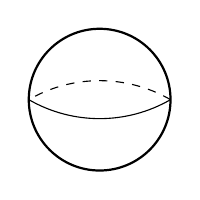
\begin{tikzpicture}[scale=0.9]
            \coordinate (A) at (0,0,0);
            \coordinate (B) at (-1,0,0);
            \coordinate (C) at (1,0,0);

            \filldraw[color=black, fill=white, thick] (A) circle (1);
            \draw (B) arc (240:300:2);
            \draw[dashed] (C) arc (60:120:2);
        \end{tikzpicture}
        %
        \hspace{2cm}
        %
        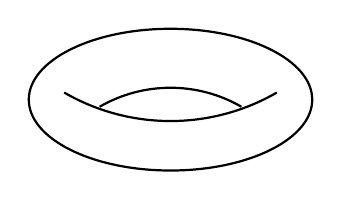
\begin{tikzpicture}[scale=0.9]
            \coordinate (A) at (0,0);
            \coordinate (B) at (-1.5,0.1);
            \coordinate (C) at (1,-0.1);

            \draw[thick] (A) ellipse (2cm and 1cm);
            \draw[thick] (B) arc (240:300:3);
            \draw[thick] (C) arc (60:120:2);
        \end{tikzpicture}
    \end{center}
    Mas adelante veremos que la homología le asigna a la esfera el grupo $\{e\}$ y al toro 
    $\Z^{2}$. En general, una superficie de genero $g$ tendrá el grupo $\Z^{2g}$.

    \item ¿Cuando $\R^{n}$ y $\R^{m}$ son homeomorfos? Si $n\neq$, el grupo de homología de 
    $\R^{n}$ será $\{e\}$ y por el contrario, para $\R^{m}$ va a ser $\Z$ y por lo tanto $R^{n}$ y
    $\R^{m}$ son homeomorfos si y solo si $n=m$.

    \item Un ejemplo particular, para el circulo se tiene que $\pi_{1}(\s^{1})=\Z$ pero 
    $\pi_{1}(\s^{2})=\{e\}$ y por lo tanto los espacios no son homeomorfos.
\end{enumerate}

\vspace{2mm}
\begin{dfn}
    Una \textbf{homotopía} entre dos funciones continuas $f,g:X\to Y$ es una función continua 
    $H:X\times[0,1]\to Y$ tal que $H(x,0)=f(x)$ y $H(x,1)=g(x)$ para todo $x\in X$.
\end{dfn}
\noindent\textbf{Notación:} La función $H_{t}:X\to Y$ esta dada por $H_{t}(x):=H(x,t)$. Una 
homotopía de $f$ a $g$ se denota por $f\sim g$.

\vspace{2mm}
\begin{prop}
    Ser homotópico es una relación de equivalencia en $\mathcal{C}(X,Y)$.
\end{prop}
\begin{proof}
    Debemos probar tres cosas
    \begin{enumerate}
        \item La relación es reflexiva. Sea $f:X\to Y$, consideramos la homotopía constante, esto
        es $H(x,t):=f(x)$ es continua ya que

        \centerline{
            \xymatrix{
                X\times[0,1] \ar[r]^-{\pi_{X}} \ar@/_0.8pc/[rr]_{H} & X \ar[r]^-{f} & Y
            }
        }
        \item Simetría. Supongamos que $f\sim g$, consideramos $H'(x,t)=H(x,1-t)$ y es continua
        por que
        
        \vspace{2mm}
        \centerline{
            \xymatrixcolsep{3pc}\xymatrix{
                X\times[0,1] \ar[r]^-{id\times(1-t)} \ar@/_1.1pc/[rr]_{H'} & X\times[0,1]
                \ar[r]^-{H} & Y
            }
        }
        \item Por último, la transitividad. Sean $f\sim g$ y $g\sim h$, Definimos 
        $H*G:X\times[0,1]\to Y$ dada por
        \begin{equation*}
            H*G(x,t):=\begin{cases}
                H(x,2t) &\quad\text{ si}\hspace{2mm}0\leq t\leq\frac{1}{2} \\
                G(x,2t-1) &\quad\text{ si}\hspace{2mm}\frac{1}{2}\leq t\leq1
            \end{cases}
        \end{equation*}
        que resulta continua por el lema del pegado.
    \end{enumerate}
\end{proof}

\newpage
\vspace{2mm}
\begin{dfn}
    Decimos que $f:X\to Y$ es una \textbf{equivalencia homotópica}, si existe $g:Y\to X$ tal que 
    $g\circ f\sim id_{X}$ y $f\circ g\sim id_{Y}$
\end{dfn}
\noindent En tal caso, $X$ e $Y$ se dicen homotópicamente equivalentes o que tienen el mismo tipo 
de homotopía y se denota por $X\sim Y$.

\vspace{2mm}
\noindent\textbf{Ejemplo:}
\begin{enumerate}
    \item Sea $f:X\to Y$ un homeomorfismo, en particular, tomando $g=f^{-1}$, se sigue que es 
    equivalencia homotópica.

    \item Se tiene que $\{0\}\sim\R^{n}$, consideremos la inclusión $i:\to\{0\}\to\R^{n}$, 
    afirmamos que es $i$ es equivalencia homotópica. En efecto, se verifica que $\pi:\R^{n}\to
    \{0\}$ es una inversa homotópica. Por un lado $\pi\circ i=id_{\{0\}}$ y por otro 
    $i\circ\pi=0$. Notamos que $H(x,t)=tx$ con $t\in[0,1]$ es una homotopía entre $0$ y 
    $id_{\R^{n}}$.

    \item Veamos que $\R^{n}\setminus\{0\}\sim\s^{n-1}$. Probaremos que la función 
    $i:\s^{n-1}\to\R^{n}\setminus\{0\}$ es equivalencia homotópica. En efecto,
    \begin{align*}
        \pi:\R^{n}\setminus\{0\} &\to \s^{n-1} \\
        x &\to \frac{x}{\abs{x}}
    \end{align*}
    es inversa homotópica. Es claro que $\pi\circ i=id_{s^{n-1}}$. Definimos
    \begin{equation*}
        H(x,t):=t\frac{x}{\abs{x}}+(1-t)x
    \end{equation*}
    Notamos que $H(x,0)=x$ y $H(x,1)=\frac{x}{\abs{x}}$, es decir, $H$ es una homotopia entre 
    $i\circ\pi$ e $id_{\R^{n}\setminus\{0\}}$. Además, se verifica que 
    $im(H)\subseteq\R^{n}\setminus\{0\}$.
\end{enumerate}

\newpage
\section{Homología}
\noindent Queremos asignarle a un espacio topológico $X$ arbitrario, grupos abelianos 
$H_{0}(X),H_{1}(X),\cdots$ tal que si $X\sim Y$, entonces $H_{i}(X)\cong H_{i}(Y)$ para todo $i$.
Ituitivamente, $H_{k}(X)$ estará generado por ciertos subespacios de $X$ de dimensión $k$.

\vspace{2mm}
\noindent Habrá una relación de equvalencia, $A,B\subseteq X$ de dimensión $k$ serán equivalentes
si hay un subespacio de $X$ de dimensión $k+1$ cuyo borde es $A\cup B$.

\vspace{2mm}
\noindent Hay que restringir la clase de espacios a una con nociones de dimensión, borde, etc. 
Estos serán los complejos simpliciales. Necesitamos, adicionalmente, un objeto algebraico que 
capture esas nociones, esto corresponde a los complejos de cadenas.

\subsection{Complejos de Cadenas}
\begin{dfn}
    Un \textbf{complejo de cadenas} es una sucesión de grupos abelianos y homomorfismos
    
    \vspace{2mm}
    \centerline{
        \xymatrix{
            \cdots \ar[r] & C_{3} \ar[r]^{\partial_{3}} & C_{2} \ar[r]^{\partial_{2}} & 
            C_{1} \ar[r]^{\partial_{1}} & C_{0} \ar[r] & 0
        }
    }
    \vspace{2mm}
    \noindent tal que $\partial_{i}\circ \partial_{i+1}=0$ para todo $i$. Se denota por 
    $(C_{\sbullet},\partial_{\sbullet})$.
\end{dfn}
\noindent\textbf{Observación:} Notemos que $\im{\partial_{i+1}}\subseteq\kr{\partial_{i}}
\subseteq C_{i}$. Dado que los grupos son abelianos, esta observación permite definir el siguiente 
objeto.

\vspace{2mm}
\begin{dfn}
    El \textbf{i-ésimo grupo de homología} de $(C_{\sbullet},\partial_{\sbullet})$ se define por
    \begin{equation*}
        H_{i}(C_{i}):=\frac{\kr{\partial_{i}}}{\im{\partial_{i+1}}}
    \end{equation*}
\end{dfn}

\vspace{2mm}
\noindent\textbf{Ejemplos:}
\begin{itemize}
    \item Si $A$ un grupo abeliano, entonces
    
    \vspace{2mm}
    \centerline{
        \xymatrix{
            \cdots \ar[r] & 0 \ar[r] & 0 \ar[r] & A \ar[r] & 0 \ar[r] & \cdots \ar[r] & 0
        }
    }
    \vspace{2mm}
    es un complejo de cadenas donde $C_{i}=A$. Entonces
    \begin{equation*}
        H_{j}(C_{\sbullet})=\begin{cases}
            0 & \quad\text{si }j\neq i \\
            A & \quad\text{si }j=i
        \end{cases}
    \end{equation*}

    \item Consideremos la cadena exacta
    
    \vspace{2mm}
    \centerline{
        \xymatrix{
            \cdots \ar[r] & 0 \ar[r] & \Z \ar[r]^{\cdot2} & \Z \ar[r]^{\pi} & \Z_{2} \ar[r] & 0
        }
    }
    \vspace{2mm}
    entonces $H_{j}(C_{\sbullet})=0$ para todo $i$.

    \item Veamos que
    
    \vspace{2mm}
    \centerline{
        \xymatrix{
            \cdots \ar[r] & \Z \ar[r]^{\cdot2} & \Z \ar[r]^{\cdot0} & \Z \ar[r] & 0
        }
    }
    \vspace{2mm}    
    es un complejo de cadenas. Los grupos de homología asociados son $H_{0}(C_{\sbullet})=\Z$, 
    $H_{1}(C_{\sbullet})=\Z_{2}$ y $H_{k}(C_{\sbullet})=0$ para $k\neq0,1$.
\end{itemize}

\begin{dfn}
    Sean $(C_{\sbullet},\partial_{\sbullet})$ y $(D_{\sbullet},\partial_{\sbullet})$ dos complejos 
    de cadenas. Un \textbf{mapeo de cadenas} es una colección de homomorfismos 
    $f_{n}:C_{n}\to D_{n}$ tal que $\partial_{n}f_{n}=f_{n-1}\partial_{n}$ para todo $n$, es 
    decir, el siguiente diagrama conmuta

    \vspace{2mm}
    \centerline{
        \xymatrix{
            C_{n} \ar[r]^{\partial_{n}} \ar[d]^{f_{n}} & C_{n-1} \ar[d]^{f_{n-1}} \\
            D_{n} \ar[r]^{\partial_{n}} & D_{n-1}
        }
    }
    \noindent y se denota por $f_{\sbullet}:C_{\sbullet}\to D_{\sbullet}$.
\end{dfn}

\vspace{2mm}
\begin{lema}
    Si $f_{\sbullet}:C_{\sbullet}\to D_{\sbullet}$ es un mapeo de cadenas, entonces la asignación 
    $f_{*}:H_{n}(C_{\sbullet})\to H_{n}(D_{\sbullet})$ dada por
    \begin{equation*}
        f_{*}([x])=[f_{n}(x)]
    \end{equation*}
    esta bien definida y es un homomorfismo de grupos.
\end{lema}
\begin{proof}
    Sea $x\in ker\partial_{n}$ entonces $\partial_{n}f_{n}(x)=f_{n-1}\partial_{n}(x)
    =f_{n-1}(0)=0$. Así, $f_{n}(x)\in\kr{\partial_{n}}$ y por tanto la expresión tiene sentido. Si
    $[x]=[y]$ entonces $x-y=\partial_{n}(z)$ para $z\in C_{n+1}$, se sigue que 
    $f_{n}(x)-f_{n}(y)=f_{n}\partial_{n+1}(z)=\partial_{n+1}f_{n+1}(z)$. Concluimos que 
    $[f_{n}(x)]=[f_{n}(y)]$.
\end{proof}

\noindent\textbf{Ejemplo:}
Consideremos la siguiente situación

\vspace{2mm}
\centerline{
    \xymatrix{
        \cdots \ar[r] & 0 \ar[r]^{0} \ar[d] & \Z \ar[r]^{3} \ar[d]^{id} & 
        \Z \ar[r]^{0} \ar[d]^{\pi} & \Z \ar[r] \ar[d]^{id} & 0 
        & C_{\sbullet} \ar[d]^{f_{\sbullet}} \\
        \cdots \ar[r] & 0 \ar[r]^{0} & \Z \ar[r]^{3} & \Z_{3} \ar[r]^{0} & \Z \ar[r] & 0 
        & D_{\sbullet}
    }
}
\vspace{2mm}
\noindent Entonces $f_{*}:H_{2}(C_{\sbullet})=0\to H_{2}(D_{\sbullet})=\Z$ es el morfismo trivial. 
Mientras que $\pi_{*}:H_{1}(C_{\sbullet})=\Z_{3}\to H_{1}(D_{\sbullet})=\Z_{3}$ es la identidad.

\vspace{2mm}
\noindent\textbf{Observación:} Sea $g_{\sbullet}:D_{\sbullet}\to G_{\sbullet}$ un mapeo de 
cadenas, entonces $(g\circ f)_{\sbullet}:C_{\sbullet}\to G_{\sbullet}$ es un mapeo de cadenas y el 
siguiente diagrama conmuta

\vspace{2mm}
\centerline{
    \xymatrix{
        H_{n}(C_{\sbullet}) \ar[rr]^{(g\circ f)_{*}} \ar[rd]^{f_{*}} & 
        & H_{n}(G_{\sbullet}) \\
        & H_{n}(D_{\sbullet}) \ar[ru]^{g_{*}}
    }
}
\vspace{2mm}
\noindent Notemos que $\partial_{n}g_{n} f_{n}=g_{n-1}\partial_{n}f_{n}=g_{n-1}f_{n-1}
\partial_{n}$. Por otro lado, tenemos que $(g\circ f)_{*}([x])=[(g\circ f)(x)]=g_{*}([f(x)])=
(g_{*}\circ f_{*})([x])$, lo que prueba la afirmación.

\begin{dfn}
    Sean $i_{\sbullet}:A_{\sbullet}\to B_{\sbullet}$ y $j_{\sbullet}:B_{\sbullet}\to C_{\sbullet}$
    dos mapeos de cadenas. Decimos que forman una sucesión exacta corta si la secuencia

    \vspace{2mm}
    \centerline{
        \xymatrix{
            0 \ar[r] & A_{n} \ar[r]^{i_{n}} & B_{n} \ar[r]^{j_{n}} & C_{n} \ar[r] & 0
        }
    }
    \vspace{2mm}
    \noindent es exacta y corta de grupos abelianos libres para todo $n\in\N$. Lo denotamos como
    $0\to A_{\sbullet}\to B_{\sbullet}\to C_{\sbullet}\to0$.
\end{dfn}

\begin{teo}[Lema de la serpiente]
    Sea $0\to A_{\sbullet}\to B_{\sbullet}\to C_{\sbullet}\to0$ una secuencia de complejos de 
    cadenas, entonces existen morfismos
    \begin{equation*}
        \delta_{n}:H_{n}(C_{\sbullet})\to H_{n-1}(A_{\sbullet})
    \end{equation*}
    tal que
    
    \vspace{2mm}
    \centerline{
        \xymatrix{
            \ar[r]^-{\delta_{n+1}} & H_{n}(A_{\sbullet}) \ar[r]^{i_{*}} 
            & H_{n}(B_{\sbullet}) \ar[r]^{j_{*}} & H_{n}(C_{\sbullet}) 
            \ar `[dl] `[l] `[llld]_{\delta_{n}} `[d] [dll] \\
            & H_{n-1}(A_{\sbullet}) \ar[r]^{i_{*}} & H_{n-1}(B_{\sbullet}) \ar[r]^{j_{*}} 
            & H_{n-1}(C_{\sbullet}) \ar[r] & \cdots \\
            & \cdots \ar[r] & H_{0}(B_{\sbullet}) \ar[r] & H_{0}(C_{\sbullet}) \ar[r] & 0 
        }
    }
\end{teo}

\begin{proof}
    Vamos a hacer un cacería de diagramas (:D). Consideremos el diagrama

    \vspace{2mm}
    \centerline{
        \xymatrix{
            & \vdots \ar[d] & \vdots \ar[d] & \vdots \ar[d] & \\
            0 \ar[r] & A_{n+1} \ar[r]^{i} \ar[d]^{\partial} & B_{n+1} \ar[r]^{j} \ar[d]^{\partial} 
            & C_{n+1} \ar[r] \ar[d]^{\partial} & 0 \\
            0 \ar[r] & A_{n} \ar[r]^{i} \ar[d]^{\partial} & B_{n} \ar[r]^{j} \ar[d]^{\partial} 
            & C_{n} \ar[r] \ar[d]^{\partial} & 0 \\
            0 \ar[r] & A_{n-1} \ar[r]^{i} \ar[d] & B_{n-1} \ar[r]^{j} \ar[d] 
            & C_{n-1} \ar[r] \ar[d] & 0 \\
            & \vdots & \vdots & \vdots &
        }
    }
    \vspace{2mm}
    \noindent Primero debemos definir $\delta_{n}:H_{n}(C_{\sbullet})\to H_{n-1}(A_{\sbullet})$.
    Sea $[c]\in H_{n}(C_{\sbullet})$ entonces $c\in\kr{\partial}\subseteq C_{n}$. Como $j$ es 
    sobre, existe $b\in B_{n}$ tal que $j(b)=c$. Consideramos $\partial b$ y notamos que
    \begin{equation*}
        j\partial(b)=\partial j(b)=\partial c=0
    \end{equation*}
    entonces existe un único $a\in A_{n-1}$ tal que $i(a)=\partial b$. Verificamos que 
    $i\partial(a)=\partial i(a)=\partial^{2}b=0$ y como $i$ es inyectiva vemos que 
    $\partial a=0$. Afirmamos que $\delta_{n}:H_{n}(C_{\sbullet})\to H_{n-1}(A_{\sbullet})$ por
    \begin{equation*}
        \delta_{n}([c])=[a]
    \end{equation*}
    cumple lo buscado. Debemos demostrar lo siguiente
    \begin{enumerate}
        \item No depende de la elección de $b$. Sea $b'$ tal que $j(b')=c$ entonces 
        $j(b'-b)=c-c=0$, existe único $a_{0}$ tal que $i(a_{0})=b'-b$. Por otro lado, existe $a'$
        tal que
        \begin{equation*}
            i(a')=\partial b'=\partial b+\partial i(a_{0})=\partial b+i\partial(a_{0})
        \end{equation*}
        entonces $i(a'-\partial a_{0})=\partial b=i(a)$, por inyectividad, $a'-\partial a_{0}=a$,
        lo que implica que $[a]=[a']$.

        \item No depende de la elección del representante de $[c]$. Sea $c'=c+\partial c''
        =j(b)+\partial j(b'')=j(b)+j\partial(b'')$, diremos $b'=b+\partial b''$, notemos que
        $\partial b'=\partial b+\partial^{2}b''=\partial b$. El mismo $a\in A_{n-1}$ satisface
        $i(a)=\partial b'$. Entonces $\delta_{n}[c]=[a]=\delta_{n}[c']$.

        \item La función $\delta_{n}$ es morfismo, es decir
        \begin{equation*}
            \delta_{n}([c]+[c'])=\delta_{n}[c]+\delta_{n}[c']
        \end{equation*}
        Notar que si $j(b)=c$ y $j(b')=c'$ entonces $j(b+b')=c+c'$, existen únicos 
        $a,a'\in A_{n-1}$ tales que $i(a+a')=\partial(b+b'')$ y así
        \begin{equation*}
            \partial_{n}([c+c'])=[a+a']=[a]+[a']
        \end{equation*}

        \item Exactitud en $H_{n}(C_{\sbullet})$ y $H_{n}(A_{\sbullet})$. Veamos que 
        $\im{j_{*}}\subseteq\kr{\delta_{n}}$. Sea $j_{*}[b]$ con $\partial b=0$. Entonces
        \begin{equation*}
            \delta_{n}j_{*}[b]=\delta_{n}[j(b)]
        \end{equation*}
        Existe único $a\in A_{n-1}$ tal que $i(a)=\partial b=0$, entonces $a=0$ y por lo tanto
        $\delta_{n}j_{*}[b]=[a]=0$. Queda ver que $\kr{\delta_{n}}\subseteq\im{j_{*}}$. Sea
        $[c]\in\kr{\delta_{n}}$ con $\partial c=0$. Por definición de $\delta_{n}$, para cada
        $b$ tal que $j(b)=c$ hay un único $a\in A_{n-1}$ tal que $i(a)=\partial b$.

        \noindent Como $\delta_{n}[c]=[a]=0$ se sigue que $a=\partial a'$ y entonces 
        $\partial b=i(a)=i\partial(a')=\partial i(a')$, así $b-i(a')\in\kr{\partial}$, es decir
        $b-i(a')$ representa una clase de homología.

        \noindent Ahora $j(b-i(a'))=j(b)=c$, por ende, $j_{*}[b-i(a')]=[c]$. Para 
        $H_{n}(A_{\sbullet})$ la demostración es similar.

        \item Exactitud en $H_{n}(B_{\sbullet})$. Sea $[a]\in\im{i_{*}}$ con $\partial a=0$, 
        entonces
        \begin{equation*}
            j_{*}i_{*}[a]=[j_{n}i_{n}(a)]=0
        \end{equation*}
        y por lo tanto $\im{i_{*}}\subseteq\kr{j_{*}}$. Sea $[b]\in\kr{j_{*}}$ con 
        $\partial b=0$, entonces $j_{*}[b]=[j(b)]=0$, lo que implica que $j(b)=\partial c'
        =\partial j(b')=j\partial(b')$, existe único $a\in A_{n-1}$ tal que $b-\partial b'=i(a)$,
        además
        \begin{equation*}
            i\partial(a)=\partial i(a)=\partial b+\partial^{2}b'=0
        \end{equation*}
        entonces $\partial a=0$. Luego $i_{*}[a]=[b]$. Concluimos que $im{i_{*}}=\kr{j_{*}}$.
    \end{enumerate}
    Lo que concluye el teorema.
\end{proof}

\begin{dfn}
    Sean $f_{\sbullet},g_{\sbullet}:C_{\sbullet}\to D_{\sbullet}$ mapeos de cadenas. Una 
    \textbf{homotopía de cadenas} es una colección de morfismos
    \begin{align*}
        h_{n}:C_{n}\to C_{n+1}\htext{tal que} \\
        f_{n}-g_{n}=\partial h_{n}+h_{n-1}\partial
    \end{align*}
    Lo denotamos como $f_{\sbullet}\sim g_{\sbullet}$.
\end{dfn}

\begin{prop}
    Sea $f_{\sbullet}\sim g_{\sbullet}$ entonces $f_{*}=g_{*}$.
\end{prop}
\begin{proof}
    Sea $[x]\in H_{n}(C_{\bullet})$, por definición, sabemos que $\partial x=0$, luego
    \begin{equation*}
        (f_{*}-g_{*})([x])=[(f-g)(x)]=[(\partial h+h\partial)(x)]=[\partial hx]=0
    \end{equation*}
    lo que prueba la afirmación.
\end{proof}

\begin{prop}[Lema del 5]
    Considerar el siguiente diagrama conmutativo
    
    \vspace{2mm}
    \centerline{
        \xymatrix{
            A_{1} \ar[r] \ar[d]^{f_{1}} & A_{2} \ar[r] \ar[d]^{f_{2}} 
            & A_{3} \ar[r] \ar[d]^{f_{3}} & A_{4} \ar[r] \ar[d]^{f_{4}} & A_{5} \ar[d]^{f_{5}} \\
            B_{1} \ar[r] & B_{2} \ar[r] & B_{3} \ar[r] & B_{4} \ar[r] & B_{5}
        }
    }

    \vspace{2mm}
    \noindent donde las filas son secuencias exactas y cada cuadrado conmuta. Si 
    $f_{1},f_{2},f_{4}$ y $f_{5}$ son isomorfismos, entonces $f_{3}$ es isomorfismo.
\end{prop}

\begin{proof}
    Por simplicidad del argumento, denotaremos los morfismos $A_{i}\to A_{i+1}$ y 
    $B_{i}\to B_{i+1}$ como $\partial$. Debido a que ambas secuencias son exactas, resulta que 
    $\partial^{2}a=\partial\circ\partial (a)=0$. Veamos que $\kr{f_{3}}=0$. Sea $a\in\kr{f_{3}}$,
    notemos que
    \begin{equation*}
        0=\partial f_{3}(a)=f_{4}\partial(a)\hhtext{entonces}\partial a=0
    \end{equation*}
    Como $a\in\kr\partial$, existe $a'\in A_{2}$ tal que $\partial a'=a$, luego 
    $\partial f_{2}(a')=f_{3}\partial(a')=f_{3}(a)=0$. Por exactitud, existe $b'\in B_{1}$ tal que 
    $\partial b'=f_{2}(a')$, puesto que $f_{1}$ es isomorfismo, existe $a''\in A_{1}$ tal que 
    $b'=f_{1}(a'')$, usando que los diagramas conmutan vemos que
    \begin{equation*}
        a''=f^{-1}_{1}(b')\hhtext{entonces}\partial a''=\partial f^{-1}_{1}(b')
        =f^{-1}_{2}\partial(b')
    \end{equation*}
    recordemos que $\partial b'=f_{2}(a')$, es decir, $\partial a''=a'$, luego 
    $0=\partial^{2}a''=\partial a'=a$.

    \vspace{2mm}
    \noindent Sea $b\in B_{3}$, consideramos $\partial b\in B_{4}$, entonces 
    $f^{-1}_{4}(\partial b)\in A_{4}$, por conmutatividad del diagrama, se sigue que
    $\partial f_{4}^{-1}(\partial b)=f_{5}^{-1}(\partial^{2}b)=0$, luego, por exactitud, existe
    $a\in A_{3}$ tal que $\partial a=f_{4}^{-1}(\partial b)$. Observemos que,
    \begin{equation*}
        \partial(f_{3}(a)-b)=\partial f_{3}(a)-\partial b=f_{4}\partial(a)-\partial b=0
    \end{equation*}
    Así, existe $b'\in B_{2}$ tal que $\partial b'=f_{3}(a)-b$, definimos 
    $a'=f_{2}^{-1}(b')\in A_{2}$, de este modo,
    \begin{equation*}
        f_{3}(a)-b=\partial b'=\partial f_{2}(a')=f_{3}(\partial a')
    \end{equation*}
    En resumen, $f_{3}(a-\partial a')=b$. Concluimos que $f_{3}$ es isomorfismo.
\end{proof}

\vspace{2mm}
\noindent Nuestro objetivo será asociar un complejo de cadenas a un espacio topológico $X$ 
arbitrario, lo que nos dara un grupo de homología para cada dimensión, además dada $f:X\to Y$ una
función continua, nos gustaría obtener un mapeo de cadenas y por tanto un homomorfismo entre los
grupos de homología de cada espacio.

\newpage
\subsection{Complejos Simpliciales}
\begin{dfn}
    Dados $n+1$ puntos $\{v_{0},\cdots,v_{n}\}\in\R^{\omega}$ son \textbf{afínmente 
    independientes}, si generan un $n-$plano afín, es decir, $\{v_{1}-v_{0},\cdots,v_{n}-v_{0}\}$
    es un conjunto linealmente independiente, esto es
    \begin{equation*}
        \sum_{i=0}^{n}t_{i}v_{i}=0\hhtext{y}\sum_{i=0}^{n}t_{i}=0
        \hhtext{entonces}t_{i}=0\text{ para todo }i
    \end{equation*}
\end{dfn}

\vspace{2mm}
\noindent\textbf{Ejemplo:} Dos puntos son afínmente independientes. Tres puntos son afínmente 
independientes si y solo si no son colineales.

\vspace{2mm}
\begin{dfn}
    Si $\{v_{0},\cdots,v_{n}\}$ son afínmente independientes, ellos definen el \textbf{n-simplejo}
    \begin{equation*}
        \sigma=\gen{v_{0},\cdots,v_{n}}=\left\{x=\sum_{i=0}^{n}t_{i}v_{i},\hspace{2mm}
        \sum_{i=0}^{n}t_{i}=1\hhtext{y}t_{i}\geq0\right\}
    \end{equation*}
\end{dfn}

\noindent Decimos que $\sigma$ es el $n-$simplejo generado por $v_{0},\cdots,v_{n}$. Los puntos 
$v_{i}$ se llaman \textbf{vértices} de $\sigma$. Una \textbf{cara} de un simplejo $\sigma$ es 
un simplejo $\tau$ generado por un subconjunto de $\{v_{0},\cdots,v_{n}\}$ y lo denotamos por 
$\tau\leq\sigma$. Si el subconjunto es propio, se dice que $\tau$ es una \textbf{cara propia}.

\vspace{2mm}
\noindent La \textbf{frontera} de un $n-$simplejo $\sigma$ es la unión de todas sus caras propias, 
se denota por $\partial\sigma$, el \textbf{interior} de $\sigma$ es $int(\sigma):=
\sigma\setminus\partial\sigma$.

\begin{center}
    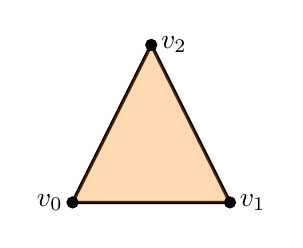
\begin{tikzpicture} %Un 2-simplejo
        \coordinate (A) at (0,0);
        \coordinate (B) at (2,0);
        \coordinate (C) at (1,2);

        \draw[very thick] (A) -- (B) -- (C) -- cycle;
        \fill[color=orange, opacity=0.3] (A) -- (B) -- (C) -- cycle;

        \filldraw (C) circle (2pt) node[anchor=west]{$v_{2}$};
        \filldraw (B) circle (2pt) node[anchor=west]{$v_{1}$};
        \filldraw (A) circle (2pt) node[anchor=east]{$v_{0}$};
    \end{tikzpicture}
\end{center}

\vspace{2mm}
\begin{dfn}
    Un \textbf{complejo simplicial} (geométrico) $K$ es un conjunto de simplejos tales que
    \begin{enumerate}
        \item Si $\sigma\in K$ y $\tau\leq\sigma$ entonces $\tau\in K$.
        \item Si $\sigma,\tau\in K$ entonces $\sigma\cap\tau=\emptyset$ ó $\sigma\cap\tau$ es una
        cara de $\sigma$ y de $\tau$.
    \end{enumerate}
\end{dfn}
\noindent El \textbf{poliedro} asociado a un complejo simplicial $K$ es 
$\abs{K}:=\bigcup_{\sigma\in K}\sigma$. Un espacio topológico $X$ se llama un poliedro si existe
un complejo simplicial $K$ y un homeomorfismo $f:\abs{K}\to X$. Al par $(K,f)$ se le llama una 
\textbf{triangulación} de $X$. Denotamos por $V_{K}$ al conjunto de vértices de los simplices.

\vspace{2mm}
\noindent\textbf{Observación:} Si $X$ es triangulable, entonces es Hausdorff por que $\abs{K}$ 
lo es.

\begin{center}
    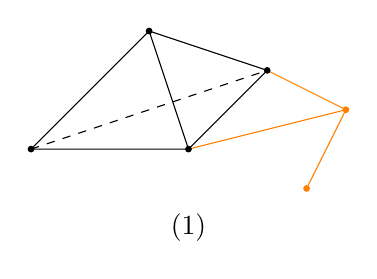
\begin{tikzpicture} %Ejemplo de complejo simplicial
        \coordinate (A) at (0,0);
        \coordinate (B) at (2,0);
        \coordinate (C) at (3,1);
        \coordinate (D) at (1.5,1.5);
        \coordinate (E) at (4,0.5);
        \coordinate (F) at (3.5,-0.5);

        \draw (A) -- (B) -- (D) -- cycle;
        \draw (D) -- (C) -- (B);
        \draw[dashed] (A) -- (C);
        \draw[color=orange] (B) -- (E) -- (C);
        \draw[color=orange] (E) -- (F);

        \filldraw (A) circle (1pt);
        \filldraw (B) circle (1pt);
        \filldraw (C) circle (1pt);
        \filldraw (D) circle (1pt);
        \filldraw[color=orange] (E) circle (1pt);
        \filldraw[color=orange] (F) circle (1pt);

        \node at (2,-1) {(1)};
    \end{tikzpicture}
    %
    \hspace{2cm}
    %
    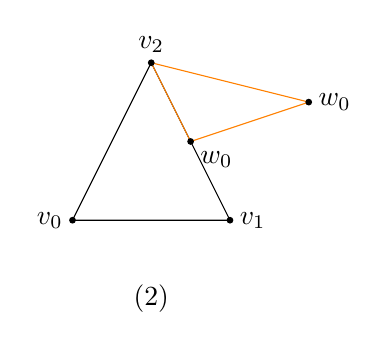
\begin{tikzpicture} %Ejemplo de un no complejo simplicial
        \coordinate (A) at (0,0);
        \coordinate (B) at (2,0);
        \coordinate (C) at (1,2);
        \coordinate (D) at (1.5,1);
        \coordinate (E) at (3,1.5);

        \draw (A) -- (B) -- (C) -- cycle;
        \draw[color=orange] (C) -- (D) -- (E) -- cycle;

        \filldraw (A) circle (1pt) node[anchor=east]{$v_{0}$};
        \filldraw (B) circle (1pt) node[anchor=west]{$v_{1}$};
        \filldraw (C) circle (1pt) node[anchor=south]{$v_{2}$};
        \filldraw (D) circle (1pt) node[anchor=north west]{$w_{0}$};
        \filldraw (E) circle (1pt) node[anchor=west]{$w_{0}$};

        \node at (1,-1) {(2)};
    \end{tikzpicture}
\end{center}
\noindent La figura $(1)$ corresponde a un complejo simplicial, mientras que la figura $(2)$ no
es un complejo simplicial ya que los simplices que la componen no se pegan bien.

\vspace{2mm}
\noindent\textbf{Ejemplo:} Consideremos el complejo simplicial $K$ formado por los simplices 
$\sigma=\gen{\pm e_{1},\pm e_{2}, \pm e_{3}}$ y sus respectivas caras. Consideremos 
$f:\abs{K}\to\s^{2}$ por $f(x):=x/\abs{x}$, entonces $(K,f)$ es una triangulación de la 
$2-$esfera.

\begin{center}
    \begin{tikzpicture}[scale=0.9] %Representación del complejo simplicial
        \coordinate (O) at (0,0);
        \coordinate (A) at (-0.5,-1);
        \coordinate (B) at (1,0);
        \coordinate (C) at (0,1);

        \draw (O) -- ($1.5*(A)$);
        \draw (O) -- ($1.5*(B)$);
        \draw (O) -- ($1.5*(C)$);

        \draw[dashed] (O) -- ($-1.5*(A)$);
        \draw[dashed] (O) -- ($-1.5*(B)$);
        \draw[dashed] (O) -- ($-1.5*(C)$);

        \draw[orange] (A) -- (B) -- (C) -- cycle;
        \draw[orange] (A) -- (B) -- ($-1*(C)$) -- cycle;
        \draw[orange] (A) -- ($-1*(B)$) -- (C) -- cycle;
        \draw[orange] ($-1*(A)$) -- (B) -- (C) -- cycle;

        \draw[orange, dashed] ($-1*(B)$) -- ($-1*(C)$);
        \draw[orange, dashed] ($-1*(B)$) -- ($-1*(A)$);
        \draw[orange, dashed] ($-1*(A)$) -- ($-1*(C)$);

        \filldraw (A) circle (1pt) node[anchor=north west]{$e_{1}$};
        \filldraw (B) circle (1pt) node[anchor=north west]{$e_{2}$};
        \filldraw (C) circle (1pt) node[anchor=south west]{$e_{3}$};
    \end{tikzpicture}
\end{center}

\vspace{2mm}
\begin{dfn}
    Sean $K$ y $L$ complejos simpliciales. Un \textbf{mapeo simplicial} de $K$ a $L$ es una 
    función $f:V_{K}\to V_{L}$ tal que si $\sigma=\gen{v_{\alpha_{0}},\cdots,v_{\alpha_{n}}}$ es
    un simplejo en $K$ entonces
    \begin{equation*}
        \{f(v_{\alpha_{0}}),\cdots,f(v_{\alpha_{n}})\}
    \end{equation*}
    genera un simplice en $L$, al cual llamamos $f(\sigma)$. Notación $f:K\to L$.
\end{dfn}

\vspace{2mm}
\noindent\textbf{Ejemplo:} Sea $\triangle^{n}=\gen{e_{1},\cdots,e_{n+1}}\subseteq\R^{n+1}
\subseteq\R^{\infty}$. Entonces las funciones $f:\triangle^{1}\to\triangle^{2}$ y 
$g:\triangle^{2}\to\triangle^{1}$ dadas por $f(e_{i})=e_{i}$ y $g(e_{1})=g(e_{3})=e_{1}$, 
$g(e_{2})=e_{2}$ son mapeos simpliciales.

\vspace{2mm}
\begin{lema}
    Sea $f:K\to L$ un mapeo simplicial. Entonces induce una función continua 
    $\abs{f}:\abs{K}\to\abs{L}$.
\end{lema}
\begin{proof}
    Sea $\sigma\in K$, digamos que $\sigma=\gen{v_{\alpha_{0}},\cdots,v_{\alpha_{n}}}$ y Definimos
    \begin{align*}
        f_{\sigma}:\sigma &\to \abs{L} \\
        \sum_{i=0}^{k}t_{i}v_{i} &\to \sum_{i=0}^{k}t_{i}f(v_{i})
    \end{align*}
    que es continua por que es lineal en los $t_{i}$. Se observa que si $\tau\leq\sigma$ entonces
    $f_{\tau}=f_{\sigma}\big|_{\tau}$. Ahora tomamos $\sigma$ y $\sigma'$, entonces
    \begin{equation*}
        f_{\sigma}\big|_{\sigma\cap\sigma'}=f_{\sigma\cap\sigma'}
        =f_{\sigma'}\big|_{\sigma\cap\sigma'}
    \end{equation*}
    entonces $\abs{f}:=\bigcup_{\sigma\in K}f_{\sigma}$ es una función continua de $\abs{K}$ en 
    $\abs{L}$.
\end{proof}
\noindent Sea $g:L\to J$ un mapeo simplicial, entonces $g\circ f$ es mapeo simplicial, ya que $f$
mapea vértices de un simplice a vértices de un simplice y del mismo modo lo hace $g$, además se 
tiene lo siguiente
\begin{equation*}
    \abs{g\circ f}(x)=\abs{g\circ f}\left(\sum t_{i}v_{\alpha_{i}}\right)
    =\sum t_{i}(g\circ f)(v_{\alpha_{i}})=\sum t_{i}g(f(v_{\alpha_{i}}))=(\abs{g}\circ\abs{f})(x)
\end{equation*}
es decir, $\abs{g\circ f}=\abs{g}\circ\abs{f}$. Un mapeo simplicial puede ser definido también 
como una función continua $f:\abs{K}\to\abs{L}$ que manda vértices en vértices y es lineal en sus 
caras.

\vspace{2mm}
\begin{dfn}
    Sea $x\in\abs{K}$. El \textbf{portador} de $x$ es el simplejo de $K$ mas pequeño (en términos
    de inclusión) que contiene a $x$. Se denota por $carr(x)$.
\end{dfn}

\vspace{2mm}
\begin{dfn}
    Sea $w\in V_{K}$. El conjunto $St_{K}(w):=\{x\in\abs{K}:w\in carr(x)\}$ le decimos la 
    \textbf{estrella de $w$}.
\end{dfn}

\vspace{2mm}
\noindent\textbf{Ejemplo:} Veamos el siguiente complejo
\begin{center}
    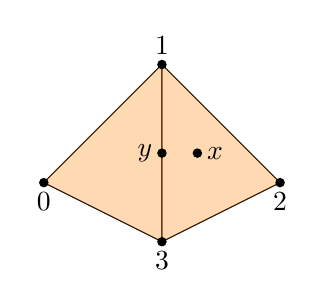
\begin{tikzpicture}[scale=1.5] %Ejemplo concreto del portador
        \coordinate (O) at (0,0);
        \coordinate (A) at (1,0.5);
        \coordinate (B) at (-1,0.5);
        \coordinate (C) at (0,1.5);

        \draw (O) -- (A) -- (C) -- cycle;
        \draw (O) -- (B) -- (C) -- cycle;

        \fill[color=orange, opacity=0.3] (O) -- (A) -- (C) -- cycle;
        \fill[color=orange, opacity=0.3] (O) -- (B) -- (C) -- cycle;

        \filldraw (B) circle (1pt) node[anchor=north]{$0$};
        \filldraw (A) circle (1pt) node[anchor=north]{$2$};
        \filldraw (O) circle (1pt) node[anchor=north]{$3$};
        \filldraw (C) circle (1pt) node[anchor=south]{$1$};

        \filldraw (0,0.75) circle (1pt) node[anchor=east]{$y$};
        \filldraw (0.3,0.75) circle (1pt) node[anchor=west]{$x$};
    \end{tikzpicture}
\end{center}
Entonces $carr(y)=\gen{1,3}$, $carr(x)=\gen{1,2,3}$ y $carr(3)=\gen{3}$.

\vspace{2mm}
\noindent\textbf{Observación:} Notemos que $y\in carr(x)$ si y solo si $carr(y)\subseteq carr(x)$.
Sea $\sigma\in K$, entonces $\sigma=carr(x)$ si y solo si $x\in int(\sigma)$, esto es una 
caracterización útil del portador.

\vspace{2mm}
\noindent En efecto, si $\sigma=carr(x)$, supongamos, por contradicción, que $x\in\partial\sigma$,
entonces $x\in\tau<\sigma$, como $K$ es complejo, $\tau\in K$. Por otro lado, si 
$x\in int(\sigma)$, sea $\tau\in K$ tal que $x\in\tau$, luego $\tau\cap\sigma$ es una cara de 
$\sigma$, pero $x\in\tau\cap\sigma$ lo que implica que $\sigma=\tau\cap\sigma\subseteq\tau$, es
decir, $\sigma=carr(x)$.

\noindent Por otro lado, usando lo anterior vemos que $St_{K}(w)=\bigcup_{w\in\sigma\in K}
int(\sigma)$, entonces la estrella de un vértice es un abierto en $\abs{K}$.

\vspace{2mm}
\begin{prop}
    Sea $g:K\to L$ un mapeo simplicial, entonces $g(carr(x))=carr(g(x))$.
\end{prop}
\begin{proof}
    Por la observación anterior, basta probar que $g(x)\in int(g(carr(x)))$, sean $v_{i}\in V_{K}$
    tales que $\gen{v_{1},\cdots,v_{n}}=carr(x)$, luego
    \begin{equation*}
        x=\sum_{i=1}^{n}t_{i}v_{i}\htext{donde}t_{i}>0\text{ para todo }i\text{, entonces}
        \hspace{4mm}g(x)=\sum_{i=0}^{n}t_{i}g(v_{i})\in g(carr(x))
    \end{equation*}
    como $t_{i}>0$ vemos que $g(x)\in int(g(carr(x)))$.
\end{proof}

\begin{dfn}
    Sea $f:\abs{K}\to\abs{L}$ una función continua. Una \textbf{aproximación simplicial} a $f$ es 
    un mapeo simplicial $g:K\to L$ tal que
    \begin{equation*}
        g(x)\in carr(f(x))\text{ para todo }x\in\abs{K}
    \end{equation*}
\end{dfn}
\noindent\textbf{Ejemplo:} Se definen los siguientes complejos simpliciales,
\begin{center}
    \begin{tikzpicture} %Complejo simplicial K%
        \coordinate (A) at (1,0);
        \coordinate (B) at ({sqrt(2)/2},{sqrt(2)/2});
        \coordinate (C) at (0,1);
        \coordinate (D) at (-{sqrt(2)/2},{sqrt(2)/2});
        \coordinate (E) at (-1,0);
        \coordinate (F) at (-{sqrt(2)/2},-{sqrt(2)/2});
        \coordinate (G) at (0,-1);
        \coordinate (H) at ({sqrt(2)/2},-{sqrt(2)/2});

        \draw (A) -- (B) -- (C) -- (D) -- (E) -- (F) -- (G) -- (H) -- cycle;

        \filldraw (A) circle (1pt) node[anchor=west]{$v_{0}$};
        \filldraw (B) circle (1pt) node[anchor=south west]{$v_{1}$};
        \filldraw (C) circle (1pt) node[anchor=south]{$v_{2}$};
        \filldraw (D) circle (1pt) node[anchor=south east]{$v_{3}$};
        \filldraw (E) circle (1pt) node[anchor=east]{$v_{4}$};
        \filldraw (F) circle (1pt) node[anchor=north east]{$v_{5}$};
        \filldraw (G) circle (1pt) node[anchor=north]{$v_{6}$};
        \filldraw (H) circle (1pt) node[anchor=north west]{$v_{7}$};

        \filldraw ($(O)-(2,1)$) node{K};
    \end{tikzpicture}
    %
    \hspace{2cm}
    %
    \begin{tikzpicture} %Complejo simplicial L
        \coordinate (A) at (1,0);
        \coordinate (B) at (0,1);
        \coordinate (C) at (-1,0);
        \coordinate (D) at (0,-1);

        \draw (A) -- (B) -- (C) -- (D) -- cycle;

        \filldraw (A) circle (1pt) node[anchor=west]{$w_{0}$};
        \filldraw (B) circle (1pt) node[anchor=south]{$w_{1}$};
        \filldraw (C) circle (1pt) node[anchor=east]{$w_{2}$};
        \filldraw (D) circle (1pt) node[anchor=north]{$w_{3}$};

        \filldraw ($(O)-(2,1)$) node{L};
    \end{tikzpicture}
\end{center}
El poliedro asociado a cada complejo es $\s^{1}$, consideramos la función continua $f(z)=z^{2}$,
una aproximación simplicial es $g(v_{i})=g(v_{i+4})=w_{i}$ para $0\leq i\leq3$.

\vspace{2mm}
\begin{dfn}
    Sea $K$ un complejo simplicial. La \textbf{primera subdivisión baricéntrica $K'$ de $K$} es el 
    complejo simplicial $K'$ cuyos
    \begin{itemize}
        \item Vértices son los baricentros $\hat{\sigma}$ de los simpleces $\sigma$ de $K$.
        \item Un $n-$simplice de $K'$ es 
        $\gen{\hat{\sigma_{0}},\hat{\sigma_{1}},\cdots,\hat{\sigma_{n}}}$ si 
        $\sigma_{0}<\sigma_{1}<\cdots<\sigma_{n}$ (Son caras propias).
    \end{itemize}
    Una $r-$ésima división baricéntrica se define recursivamente $K^{(r)}:=(K^{(r-1)})'$.
    Recordemos que si $\sigma=\gen{v_{0},\cdots,v_{n}}$ entonces 
    $\hat{\sigma}=\frac{1}{n+1}\sum v_{i}$.
\end{dfn}

\vspace{2mm}
\begin{prop}
    Sea $K$ un complejo simplicial entonces $\abs{K'}=\abs{K}$.
\end{prop}

\vspace{2mm}
\noindent\textbf{Ejemplo:} Algunos ejemplos de división baricéntrica de dos simplices.
\begin{center}
    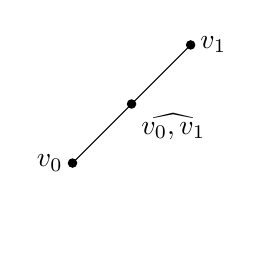
\begin{tikzpicture}[scale=1.5] %División de un 1-simplice
        \coordinate (A) at (0,0);
        \coordinate (B) at (1,1);
        \coordinate (C) at (0.5,0.5);

        \draw (A) -- (B);

        \filldraw (A) circle (1pt) node[anchor=east]{$v_{0}$};
        \filldraw (B) circle (1pt) node[anchor=west]{$v_{1}$};
        \filldraw (C) circle (1pt) node[anchor=north west]{$\widehat{\gen{v_{0},v_{1}}}$};

        \filldraw (0,-0.5) node[]{};
    \end{tikzpicture}
    %
    \hspace{2cm}
    %
    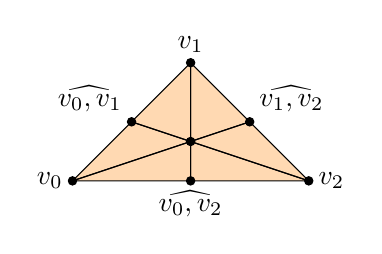
\begin{tikzpicture}[scale=1.5] %División de un 2-simplice
        \coordinate (A) at (-1,0);
        \coordinate (B) at (1,0);
        \coordinate (C) at (0,1);

        \coordinate (D) at (0,0);
        \coordinate (E) at (0.5,0.5);
        \coordinate (F) at (-0.5,0.5);

        \coordinate (G) at (0,{1/3});

        \fill[color=orange, opacity=0.3] (A) -- (B) -- (C) -- cycle;
        
        \draw (A) -- (D) -- (G) -- cycle;
        \draw (A) -- (F) -- (G) -- cycle;

        \draw (B) -- (D) -- (G) -- cycle;
        \draw (B) -- (E) -- (G) -- cycle;

        \draw (C) -- (E) -- (G) -- cycle;
        \draw (C) -- (F) -- (G) -- cycle;

        \filldraw (A) circle (1pt) node[anchor=east]{$v_{0}$};
        \filldraw (B) circle (1pt) node[anchor=west]{$v_{2}$};
        \filldraw (C) circle (1pt) node[anchor=south]{$v_{1}$};

        \filldraw (D) circle (1pt) node[anchor=north]{$\widehat{\gen{v_{0},v_{2}}}$};
        \filldraw (E) circle (1pt) node[anchor=south west]{$\widehat{\gen{v_{1},v_{2}}}$};
        \filldraw (F) circle (1pt) node[anchor=south east]{$\widehat{\gen{v_{0},v_{1}}}$};
        \filldraw (G) circle (1pt);
    \end{tikzpicture}
\end{center}
donde el punto central del segundo ejemplo es $\widehat{\gen{v_{0},v_{1},v_{2}}}$.

\newpage
\subsection{Homología Simplicial}
\noindent Dado $K$ un complejo simplicial finito, esto es, que tiene un número finito de vértices. 
Elegimos un orden total en el conjunto de vértices, digamos $v_{0}<v_{1}<\cdots<v_{n}$.

\vspace{2mm}
\begin{dfn}
    (\textbf{Complejo de cadenas simplicial}) Consideremos los grupos abelianos
    \begin{equation*}
        C_{n}(K):=\left\{\sum n_{\sigma}\sigma:\sigma=\gen{v_{\alpha_{0}},\cdots,v_{\alpha_{n}}}
        \text{ tal que}\hspace{2mm}v_{\alpha_{0}}<\cdots<v_{\alpha_{n}}
        \text{ y}\hspace{2mm}n_{\sigma}\in\Z
        \text{ nulo salvo finitos casos}\right\}
    \end{equation*}
    y los diferenciales $\partial_{n}:C_{n}(K)\to C_{n-1}(K)$ se define en la base por
    \begin{equation*}
        \partial_{n}\gen{v_{\alpha_{0}},\cdots,v_{\alpha_{n}}}
        =\sum_{i=0}^{n}(-1)^{i}\gen{v_{\alpha_{0}},\cdots,\widehat{v_{\alpha_{i}}},
        \cdots,v_{\alpha_{n}}}
    \end{equation*}
    donde $\gen{v_{\alpha_{0}},\cdots,\widehat{v_{\alpha_{i}}},\cdots,v_{\alpha_{n}}}:=
    \gen{v_{\alpha_{0}},\cdots,v_{\alpha_{i-1}},v_{\alpha_{i+1}},\cdots,v_{\alpha_{n}}}$. Se 
    extiende linealmente al resto del grupo.
\end{dfn}

\vspace{2mm}
\begin{teo}
    La tupla $(C_{\sbullet}(K),\partial_{\sbullet})$ es un complejo de cadenas, además, la 
    homología del complejo no depende del orden en el conjunto de vértices.
\end{teo}

\vspace{2mm}
\begin{dfn}
    Sea $K$ un complejo simplicial finito. El \textbf{i-ésimo grupo de homología simplicial} de 
    $K$ es
    \begin{equation*}
        H_{i}(K):=H_{i}(C_{\sbullet}(K))=\frac{\kr{\partial_{i}}}{\im{\partial_{i+1}}}
    \end{equation*}
\end{dfn}

\noindent\textbf{Ejemplos:}
\begin{enumerate}
    \item Sea $K=\{\gen{v_{0},v_{1}},\{v_{0}\},\{v_{1}\}\}$ y consideramos el 
    orden $v_{0}<v_{1}$. El complejo corresponde a un segmento de recta, notemos que 
    $3v_{0}-5v_{1}\in C_{0}(K)$, con la identificación $v_{0}=(1,0)$ y $v_{1}=(0,1)$ vemos que 
    $C_{0}(K)\cong\Z\oplus\Z$, esta identificación no es canónica, es decir, depende de la base 
    que escojamos y sus imagenes correspondientes.

    \vspace{2mm}
    \noindent Por otro lado, $C_{1}(K)\cong\Z$ con la identificación $\gen{v_{0},v_{1}}=1$. 
    Adicionalmente, se tiene que $C_{i}(K)=0$ para $i>1$. Luego,

    \vspace{2mm}
    \centerline{
        \xymatrix{
            0 \ar[r] & C_{1}(K) \ar[r]^{\partial_{1}} & C_{0}(K) \ar[r]^-{0} & 0
        }
    }
    \vspace{2mm}
    \noindent donde $\partial_{1}\gen{v_{0},v_{1}}=v_{1}-v_{2}\in C_{0}(K)$. Con las 
    identificaciones que hicimos resulta que $\partial_{1}(1)=(-1,1)$. De este modo queda la 
    cadena

    \vspace{2mm}
    \centerline{
        \xymatrix{
            0 \ar[r] & \Z \ar[r]^-{\partial_{1}} & \Z\oplus\Z \ar[r]^-{0} & 0
        }
    }
    \vspace{2mm}
    \noindent Así $H_{0}(K)\cong\Z$, $H_{1}(K)=0$, $H_{i}(K)=0$ para $i>0$.

    \item Sean $v_{0},v_{1},v_{2}$ puntos no colineales. Consideramos $\sigma=\gen
    {v_{0},v_{1},v_{2}}$ y $K:=\{\tau\leq\sigma\}$ definimos el orden $v_{0}<v_{1}<v_{2}$. Notemos
    que
    \begin{align*}
        C_{0}(K) &= \Z\{v_{0},v_{1},v_{2}\} \\
        C_{1}(K) &= \Z\{\gen{v_{0},v_{1}},\gen{v_{1},v_{2}},\gen{v_{0},v_{2}}\} \\
        C_{2}(K) &= \Z\{\gen{v_{0},v_{1},v_{2}}\}
    \end{align*}
    Entonces $\partial_{0}=0$,
    \begin{equation*}
        \partial_{1}=\begin{cases}
            \partial\gen{v_{0},v_{1}}=v_{1}-v_{0} \\
            \partial\gen{v_{1},v_{2}}=v_{2}-v_{1} \\
            \partial\gen{v_{0},v_{3}}=v_{3}-v_{0}
        \end{cases}\hhtext{y}
        \partial_{2}\gen{v_{0},v_{1},v_{2}}=\gen{v_{1},v_{2}}-\gen{v_{0},v_{2}}+\gen{v_{0},v_{1}}
    \end{equation*}
    Realizando las identificaciones $v_{i}=e_{i+1}$ para $i=0,1,2$, $\gen{v_{0},v_{1},v_{2}}=1$,
    $\gen{v_{0},v_{1}}=e_{1},\gen{v_{1},v_{2}}=e_{2}$ y $\gen{v_{0},v_{2}}=e_{3}$ resulta que
    $C_{0}(K)\cong\Z^{3},C_{1}(K)\cong\Z^{3}$ y $C_{2}(K)\cong\Z$. Tenemos
    
    \vspace{2mm}
    \centerline{
        \xymatrix{
            \cdots \ar[r] & 0 \ar[r] & C_{2}(K) \ar[r]^{\partial_{2}} & C_{1}(K) 
            \ar[r]^{\partial_{1}} & C_{0}(K) \ar[r] & 0
        }
    }
    \vspace{2mm}
    donde
    \begin{equation*}
        \partial_{2}=\begin{pmatrix}
            1 \\ 1 \\ -1
        \end{pmatrix}
        \hhtext{y}
        \partial_{1}=\begin{pmatrix}
            -1 & 0 & -1 \\ 1 & -1 & 0 \\ 0 & 1 & 1
        \end{pmatrix}
    \end{equation*}

    Claramente $H_{i}(K)=0$ para $i>2$. Además, $\kr{\partial_{2}}$, entonces $H_{2}(K)=0$. 
    Notemos que $\im{\partial_{2}}\cong\Z$ y $\kr{\partial_{1}}\cong\Z$, luego $H_{1}(K)=0$. Por
    otro lado, $\im{\partial_{1}}\cong\Z^{2}$. Por ende $H_{0}(K)\cong\Z$.
\end{enumerate}

\vspace{2mm}
\noindent\textbf{Comentario:} Se invita a calcular la homología de un $n-$simplejo. Hasta ahora 
hemos definido todo respecto a $\Z$, pero se puede definir homología simplicial de manera análoga 
para cualquier anillo $R$.

\vspace{2mm}
\begin{lema}
    Sea $f:K\to L$ un mapeo simplicial, definimos los morfismos
    \begin{align*}
        f_{n}:C_{n}(K) &\to C_{n}(L) \\
        \gen{v_{\alpha_{0}},\cdots,v_{\alpha_{n}}} &\to \begin{cases}
            sign(\varphi)\gen{f(v_{\varphi(\alpha_{0})}),\cdots,f(v_{\varphi(\alpha_{n})})} 
            &\quad\text{ si son distintos} \\
            0 &\quad\text{ si no lo son}
        \end{cases}
    \end{align*}
    donde $\varphi$ es una permutación tal que $f(v_{\varphi(\alpha_{0})})<\cdots
    <f(v_{\varphi(\alpha_{n})})$. Entonces, la colección, es un mapeo de cadena.
\end{lema}

\noindent Por lo tanto, $f$ induce un morfismo entre los grupos de homología de los complejos
simpliciales

\vspace{2mm}
\noindent\textbf{Ejemplo:} Definimos los siguientes complejos simpliciales
\begin{center}
    \begin{tikzpicture} %Complejo simplicial K%
        \coordinate (O) at (0,0);
        \filldraw[color=black, fill=white, thick] (O) circle (1);
        
        \coordinate (A) at (1,0);
        \coordinate (B) at ({sqrt(2)/2},{sqrt(2)/2});
        \coordinate (C) at (0,1);
        \coordinate (D) at (-{sqrt(2)/2},{sqrt(2)/2});
        \coordinate (E) at (-1,0);
        \coordinate (F) at (-{sqrt(2)/2},-{sqrt(2)/2});
        \coordinate (G) at (0,-1);
        \coordinate (H) at ({sqrt(2)/2},-{sqrt(2)/2});

        \draw (A) -- (B) -- (C) -- (D) -- (E) -- (F) -- (G) -- (H) -- cycle;

        \filldraw (A) circle (1pt) node[anchor=west]{$v_{0}$};
        \filldraw (B) circle (1pt) node[anchor=south west]{$v_{1}$};
        \filldraw (C) circle (1pt) node[anchor=south]{$v_{2}$};
        \filldraw (D) circle (1pt) node[anchor=south east]{$v_{3}$};
        \filldraw (E) circle (1pt) node[anchor=east]{$v_{4}$};
        \filldraw (F) circle (1pt) node[anchor=north east]{$v_{5}$};
        \filldraw (G) circle (1pt) node[anchor=north]{$v_{6}$};
        \filldraw (H) circle (1pt) node[anchor=north west]{$v_{7}$};

        \filldraw ($(O)-(2,1)$) node{K};
    \end{tikzpicture}
    %
    \hspace{2cm}
    %
    \begin{tikzpicture} %Complejo simplicial L
        \coordinate (O) at (0,0);
        \filldraw[color=black, fill=white, thick] (O) circle (1);

        \coordinate (A) at (1,0);
        \coordinate (B) at (0,1);
        \coordinate (C) at (-1,0);
        \coordinate (D) at (0,-1);

        \draw (A) -- (B) -- (C) -- (D) -- cycle;

        \filldraw (A) circle (1pt) node[anchor=west]{$w_{0}$};
        \filldraw (B) circle (1pt) node[anchor=south]{$w_{1}$};
        \filldraw (C) circle (1pt) node[anchor=east]{$w_{2}$};
        \filldraw (D) circle (1pt) node[anchor=north]{$w_{3}$};

        \filldraw ($(O)-(2,1)$) node{L};
    \end{tikzpicture}
\end{center}
Para cada complejo se da el orden que sigue $v_{0}<v_{1}<\cdots<v_{7}$ y $w_{0}<w_{1}<w_{2}<w_{3}$ 
y definimos $f:K\to L$ por $f(v_{i})=f(v_{i+4})=w_{i}$ para $i=0,1,2,3$. Veamos quien es 
$f_{*}:H_{1}(K)\to H_{1}(L)$. En primer lugar, sabemos que
\begin{equation*}
    H_{1}(K)=ker(C_{1}(K)\to C_{0}(K))=ker\begin{pmatrix}
        -1 & 0 & 0 & -1 \\ 1 & -1 & 0 & 0 \\ 0 & 1 & -1 & 0 \\ 0 & 0 & 1 & 1
    \end{pmatrix}=\gen{\begin{pmatrix}
        1 \\ 1 \\ 1 \\ -1
    \end{pmatrix}}\cong\Z
\end{equation*}
Similarmente $H_{1}(K)\cong\Z$. Entonces
\begin{equation*}
    f_{*}(\gen{v_{0},v_{1}}+\cdots+\gen{v_{6},v_{7}}-\gen{v_{0},v_{7}})
    =2(\gen{w_{0},w_{1}}+\gen{w_{1},w_{2}}+\gen{w_{2},w_{3}}-\gen{w_{0},w_{3}})
\end{equation*}
luego $f_{*}:H_{1}(K)\xrightarrow{\cdot2} H_{1}(L)$. Por otro lado, notemos que 
$H_{0}(K)\cong H_{0}(L)\cong\Z$, ya que todo par de vértices en el complejo esta conectado por una
secuencia de aristas, luego $f_{*}([v_{0}])=[w_{0}]$, entonces 
$f_{*}:H_{0}(K)\xrightarrow{} H_{0}(L)$ es isomorfismo.

\vspace{2mm}
\begin{teo}[Mayer-Vietoris]
    Sea $K$ un complejo simplicial y $M,N$ subcomplejos de $K$ que cubren a $K$, es decir, 
    $M\cup N=K$. Se tienen los mapeos
    
    \centerline{
        \xymatrix{
            M\cap N \ar[d]^-{i_{M}} \ar[r]^-{i_{N}} & N \ar[d]^-{j_{N}} \\
            M \ar[r]^-{j_{M}} & K
        }
    }

    \vspace{2mm}
    Existen morfismos $\delta_{n}:H_{n}(K)\to H_{n-1}(K)$ tales que la secuencia

    \centerline{
        \xymatrixcolsep{3pc}\xymatrix{
            \ar[r]^-{\delta_{n+1}} & H_{n}(M\cap N) \ar[r]^-{i_{M*}\oplus i_{N*}} 
            & H_{n}(M)\oplus H_{n}(N) \ar[r]^-{j_{M*}-j_{N*}} & H_{n}(K) 
            \ar `[dl] `[l] `[llld]_{\delta_{n}} `[d] [dll] \\
            & H_{n-1}(M\cap N) \ar[r]^-{i_{M*}\oplus i_{N*}} 
            & H_{n-1}(M)\oplus H_{n-1}(N) \ar[r]^-{j_{M*}-j_{N*}} & H_{n-1}(K) \ar[r] & \cdots \\
            & \cdots \ar[r] & H_{0}(M)\oplus H_{0}(N) \ar[r]^-{j_{M*}-j_{N*}} 
            & H_{0}(K) \ar[r] & 0
        }
    }
    es exacta.
\end{teo}

\begin{proof}
    Verificaremos que
    
    \centerline{
        \xymatrixcolsep{3pc}\xymatrix{
            0 \ar[r] & C_{n}(M\cap N) \ar[r]^-{i_{M}\oplus i_{N}} 
            & C_{n}(M)\oplus C_{n}(N) \ar[r]^-{j_{M}-j_{N}} & C_{n}(K) \ar[r] & 0
        }
    }

    \vspace{2mm}
    es una secuencia exacta corta de grupos abelianos para todo $n\in\N$. En efecto, como $C_{n}$
    es libremente generado por los $n-$simplices e $i$ es inyectiva, entonces 
    $i_{M*}\oplus i_{N*}$ es inyectiva. Además, $j_{M*}-j_{N*}$ es sobreyectiva por hipotesis y
    es directo que $\im{i_{M*}\oplus i_{N*}}\subseteq\kr{j_{M*}-j_{N*}}$. Resta ver que
    \begin{equation*}
        \kr{j_{M*}-j_{N*}}\subseteq\im{i_{M*}\oplus i_{N*}}
    \end{equation*}
    Sea $(x,y)\in\kr{j_{M*}-j_{N*}}$ entonces $j_{M*}(x)=j_{N*}(y)$, es decir, $x$ e $y$ se 
    escriben como suma de simplices en $N$ y $M$ respectivamente, entonces 
    $(x,y)\in\im{i_{M*}\oplus i_{N*}}$. Así, usando el lema de la serpiente, concluimos.
\end{proof}

\noindent\textbf{Ejemplo:}
Consideremos la siguiente situación
\begin{center}
    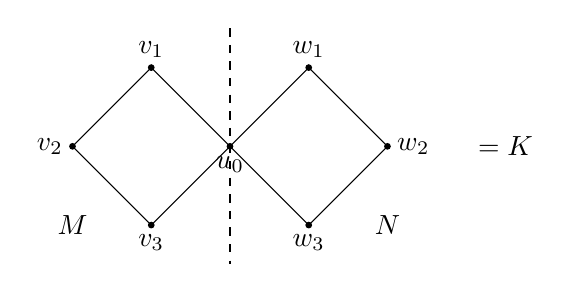
\begin{tikzpicture} %Ejemplo de Mayer Vietoris
        \coordinate (O) at (0,0);
        
        \coordinate (A) at (-1,1);
        \coordinate (B) at (-2,0);
        \coordinate (C) at (-1,-1);

        \coordinate (D) at (1,1);
        \coordinate (E) at (2,0);
        \coordinate (F) at (1,-1);

        \draw (O) -- (A) -- (B) -- (C) -- cycle;
        \draw (O) -- (D) -- (E) -- (F) -- cycle;
        \filldraw (O) circle (1pt) node[anchor=north]{$u_{0}$};
        
        \filldraw (A) circle (1pt) node[anchor=south]{$v_{1}$};
        \filldraw (B) circle (1pt) node[anchor=east]{$v_{2}$};
        \filldraw (C) circle (1pt) node[anchor=north]{$v_{3}$};

        \filldraw (D) circle (1pt) node[anchor=south]{$w_{1}$};
        \filldraw (E) circle (1pt) node[anchor=west]{$w_{2}$};
        \filldraw (F) circle (1pt) node[anchor=north]{$w_{3}$};

        \draw[dashed] (0,1.5) -- (0,-1.5);
        \filldraw (-2,-1) node{$M$};
        \filldraw (2,-1) node{$N$};
        \filldraw (3.5,0) node{$=K$};
    \end{tikzpicture}
\end{center}
Notemos que $H_{1}(M)\cong\Z$ y $H_{1}(N)\cong\Z$, además $M\cap N=\{u_{0}\}$, entonces usando
mayer vietoris nos queda que

\vspace{2mm}
\centerline{
    \xymatrix{
        0 \ar[r] & 0 \ar[r] & \Z\oplus\Z \ar[r] & H_{1}(K) 
        \ar `[dl] `[l] `[llld] `[d] [dll] \\
        & \Z \ar[r]^-{\varphi} & \Z\oplus\Z \ar[r]^{\phi} & H_{0}(K) \ar[r] & 0
    }
}

\vspace{2mm}
\noindent Para $i>2$ notamos que $H_{i}(K)=0$, por otro lado el morfismo $\varphi(1)=(1,1)$ ya que
manda generador en generador, esto por que todo par de puntos en $M$ y $N$ estan relacionados por
un camino de aristas. De este modo,
\begin{equation*}
    H_{0}(K)\cong\frac{\Z\oplus\Z}{\ker{\phi}}=\frac{\Z\oplus\Z}{\im{\varphi}}
    \cong\frac{\Z\oplus\Z}{\Z}\cong\Z
    \hhtext{y}
    H_{1}(K)\cong\Z\oplus\Z
\end{equation*}
donde el último isomorfismo se da por que $\varphi$ es inyectiva, es decir, el morfismo 
$H_{1}(K)\to\Z$ es trivial.

\begin{teo}
    Sea $f:\abs{K}\to\abs{L}$ una función continua. Entonces $f$ induce un homomorfismo
    \begin{equation*}
        f_{*}:H_{*}(K)\to H_{*}(L)
    \end{equation*}
    tal que $(g\circ f)_{*}=g_{*}\circ f_{*}$ e $id_{*}=id_{H_{*}(K)}$, donde 
    $g:\abs{L}\to\abs{M}$ es continua.
\end{teo}

\noindent\textbf{Observación:} Con esto se tendría que $H_{*}(K)$ es invariante topológico. Se
probara en dos pasos. Veremos que toda función $f$ continua se puede ``aproximar'' a una función 
$g$ simplicial, también hay que comprobar que $f_{*}:=g_{*}$ es independiente de la función 
simplicial escogida.

\begin{teo}[Aproximación Simplicial]
    Sean $K,L$ complejos simpliciales finitos y $f:\abs{K}\to\abs{L}$ una función continua. 
    Entonces existe $r\in\N$ y una aproximación simplicial a $f$
    \begin{equation*}
        g:K^{(r)}\to L
    \end{equation*}
\end{teo}

\noindent A partir de esta aproximación simplicial, se cumplen dos propiedades importantes, que 
son
\begin{enumerate}
    \item $f$ es homotópica a $g$. Notemos que $g(x),f(x)\in carr(f(x))$, entonces el segmento 
    entre $g(x)$ y $f(x)$ está en $carr(f(x))$ porque es un conjunto convexo. Definimos
    \begin{align*}
        \abs{K}\times[0,1] &\to \abs{L}\\
        (x,t) &\to tg(x)+(1-t)f(x)
    \end{align*}

    \item Sean $f_{1}:\abs{K}\to\abs{L}$, $f_{2}:\abs{L}\to\abs{M}$ continuas y $g_{1}:K\to L$, 
    $g_{2}:L\to M$ aproximaciones simpliciales de $f_{i}$, entonces $g_{2}\circ g_{1}$ es
    aproximación simplicial de $f_{2}\circ f_{1}$.

    Se tiene que
    \begin{equation*}
        g_{2}g_{1}(x)\in g_{2}(carr(f_{1}(x)))=carr(g_{2}f_{1}(x))\subseteq carr(f_{2}f_{1}(x))
    \end{equation*}
\end{enumerate}

\begin{prop}
    Sea $id:\abs{K'}\to\abs{K}$, la función $a:V_{K'}\to V_{K}$ dada por 
    $a(\hat{\sigma})=v\in V_{\sigma}$ cumple que
    \begin{enumerate}
        \item Define una aproximación simplicial de la identidad.
        \item Toda aproximación simplicial $g:K'\to K$ de la identidad es de esta forma.
    \end{enumerate}
\end{prop}

\begin{proof}
    Veamos que $a$ es un mapeo simplicial. Sea $\sigma
    =\gen{\hat{\sigma_{0}},\cdots,\hat{\sigma_{n}}}\in K'$, entonces 
    $a(\hat{\sigma_{i}})=v_{i}\in V_{\sigma_{i}}$. Sabemos que $\sigma_{i}<\sigma_{i+1}$
    para $0\leq i\leq n-1$, lo que implica que $V_{\sigma_{i}}\subset V_{\sigma_{i+1}}$, en 
    particular, $V=\{v_{0},\cdots,v_{n}\}\subseteq V_{\sigma_{n}}$, luego, $V$ genera una cara de 
    $\sigma_{n}$, es decir, un simplice en $\abs{K}$.

    \vspace{2mm}
    Sea $x\in\abs{K'}$, sean $\hat{\sigma_{i}}\in K'$ tales que 
    $\gen{\hat{\sigma_{1}},\cdots,\hat{\sigma_{n}}}=carr(x)$, luego,
    \begin{equation*}
        x=\sum_{i=1}^{n}t_{i}\hat{\sigma_{i}}\htext{donde}t_{i}>0\text{ para todo }i
    \end{equation*}
    en particular, $t_{n}>0$, como $\hat{\sigma_{n}}=\frac{1}{n+1}\sum v_{i}$ donde 
    $\gen{v_{1},\cdots,v_{n}}=\sigma_{n}$, entonces $x$ se escribe como combinación convexa de los
    $v_{i}$ donde cada poderación es positiva, luego $x\in int(\sigma_{n})$, en otras palabras,
    $carr(id(x))=\sigma_{n}$.

    \vspace{2mm}
    Lo anterior prueba que $a$ es una aproximación de la identidad. Por otro lado, si $g$ es una
    aproximación simplicial de la identidad, entonces
    \begin{equation*}
        g(\hat{\sigma})\in carr(id(\hat{\sigma}))=\sigma
    \end{equation*}
    entonces $g(\hat{\sigma})\in V_{\sigma}$, por que $g$ es mapeo simplicial.
\end{proof}

\begin{lema}[Lema del número de Lebesgue]
    Sea $X$ un espacio métrico compacto y $\mathcal{U}$ un cubrimiento abierto de $X$. Entonces 
    existe $\delta>0$ tal que para todo $x\in X$ se tiene que $B_{\delta}(x)\subseteq U$ para 
    algún $U\in\mathcal{U}$.
\end{lema}

\vspace{2mm}
\begin{lema}
    Si $f,g:K\to L$ son aproximaciones simpliciales de alguna función continua $\abs{K}\to\abs{L}$
    entonces $g_{*}=f_{*}$.
\end{lema}

\begin{proof}
    Sea $h_{n}:C_{n}(K)\to C_{n+1}(L)$ dada por $h_{n}(\gen{v_{0},\cdots,v_{n}})
    =\sum_{i=0}^{n}(-1)^{i}\sigma_{i}$ donde
    \begin{equation*}
        \sigma_{i}=\begin{cases}
            sign(\varphi_{i})\gen{f(v_{\varphi_{i}(0)}),\cdots,
            f(v_{\varphi_{i}(i)}),g(v_{\varphi_{i}(i)}),\cdots,g(v_{\varphi_{i}(n)})} 
            &\quad\text{si son distintos} \\
            0 &\quad\text{si no lo son}
        \end{cases}
    \end{equation*}
    y $\varphi_{i}$ es una permutación tal que $f(v_{\varphi_{i}(0)})<\cdots<f(v_{\varphi_{i}(i)})
    <g(v_{\varphi_{i}(i)})<\cdots<g(v_{\varphi_{i}(n)})$. Así, la colección de morfismos 
    $(h_{n})_{n}$ define una homotopía de cadenas entre $f$ y $g$.
\end{proof}

\vspace{2mm}
\begin{lema}
    Sea $a:K'\to K$ una aproximación simplicial de $id:\abs{K'}\to\abs{K}$. Entonces 
    $a_{*}:H_{i}(K')\to H_{i}(K)$ es un isomorfismo para todo $n\in\N$.
\end{lema}

\begin{proof}
    Procederemos por doble inducción en
    \begin{equation*}
        m=dim\hspace{1mm}K
        \hhtext{y}
        n=\#\text{de simplices de K de dim maximal}
    \end{equation*}
    Supongamos que $m=0$, es directo que $a_{*}$ es isomorfismo. Por otro lado, si $n=1$, entonces
    $K$ es un simplice
\end{proof}

\noindent Si iteramos, $a_{r}:K^{(r)}\to K$ entonces $a_{r*}:H_{n}(K^{(r)})\to H_{n}(K)$ es 
isomorfismo para todo $n\in\N$.

\begin{teo}
    Sea $f:\abs{K}\to\abs{L}$ una función continua, entonces el homomorfismo
    \begin{equation*}
        f_{*}:=s_{*}\circ a_{r*}^{-1}:H_{n}(K)\to H_{n}(L)
    \end{equation*}
    donde $s$ es aproximación simplicial de $f$. Cumple que
    \begin{enumerate}
        \item No depende de $s$ ni de $r$.
        \item Si $g:\abs{L}\to\abs{M}$ es continua, entonces $(f\circ g)_{*}=f_{*}\circ g_{*}$.
    \end{enumerate}
\end{teo}

\begin{proof}
    (Pendiente)
\end{proof}

\begin{lema}
    Sea $K$ un complejo simplicial finito. Entonces, existe $\varepsilon>0$ tal que si 
    $f,g:\abs{K}\to\abs{L}$ son funciones continuas que satisfacen
    \begin{equation*}
        \sup_{x\in\abs{K}}\norm{f(x)-g(x)}<\varepsilon
    \end{equation*}
    entonces $f_{*}=g_{*}$.
\end{lema}

\begin{proof}
    Sea $\{St_{L}(w)\}_{w\in V_{K}}$, que es un cubrimiento abierto de $\abs{L}$. Por el lema de
    Lebesgue, existe $\varepsilon>0$ tal que
    \begin{equation*}
        B_{2\varepsilon}(y)\subseteq St_{L}(w)\htext{para todo}w\in V_{L}
    \end{equation*}
    Sean $f,g$ continuas como en el enunciado. Consideramos $\{f^{-1}(B_{\varepsilon}(y))\}$, que
    es un cubrimiento abierto de $\abs{K}$, entonces, existe $\delta>0$ tal que
    \begin{equation*}
        f(B_{\delta}(x))\subseteq B_{\varepsilon}(y)\subseteq St_{L}(w)
        \hhtext{y}
        g(B_{\delta}(x))\subseteq B_{2\varepsilon}(y)\subseteq St_{L}(w)
    \end{equation*}
    Subdividimos $K$ de modo que
    \begin{equation*}
        \max\{\abs{v_{i}-v_{j}}:v_{i},v_{j}\in V_{K^{(r)}}\}<\frac{\delta}{2}
    \end{equation*}
    entonces
    \begin{equation*}
        f(St_{K^{(r)}}(v))\subseteq B_{\varepsilon}(y)\subseteq St_{L}(w)
        \hhtext{y}
        g(St_{K^{(r)}}(v))\subseteq B_{2\varepsilon}(y)\subseteq St_{L}(w)
    \end{equation*}
    Sea $s:V_{K^{(r)}}\to V_{L}$ dada por $s(v)=w$, luego, define una aproximación simplicial de
    $f$ y de $g$.
\end{proof}

\begin{teo}[Invarianza Homotópica]
    Sean $f,g:\abs{K}\to\abs{L}$ funciones continuas homotópicas, entonces $f_{*}=g_{*}$.
\end{teo}

\begin{proof}
    Sea $H\abs{K}\times[0,1]\to\abs{L}$ una homotopía de $f$ a $g$. Entonces $H$ es uniformemente
    continua. Sea $\varepsilon>0$ como en el lema, existe $\delta>0$ tal que
    \begin{equation*}
        \text{si }\abs{t-s}<\delta\hhtext{entonces}\norm{H(x,t)-H(x,s)}<\varepsilon
    \end{equation*}
    Sea $0=t_{0}<t_{1}<\cdots<t_{r}=1$ tal que $\abs{t_{i}-t_{i-1}}<\delta$. Definimos 
    $h_{i}(x):=H(x,t_{i})$ entonces como $\norm{h_{i}(x)-h_{i-1}(x)}<\varepsilon$ por el lema
    $(h_{i})_{*}=(h_{i-1})_{*}$.
\end{proof}

\vspace{2mm}
\begin{cor}
    Sea $f:\abs{K}\to\abs{L}$ una equivalencia homotópica, entonces $f_{*}:H_{i}(K)\to H_{i}(Y)$
    es isomorfismo para todo i.
\end{cor}

\vspace{2mm}
\begin{dfn}
    Sea $X$ un espacio topológico. Una \textbf{triangulación homotópica} es un par $(K,h)$ donde 
    $K$ es un complejo simplicial finito y $h:\abs{K}\to X$ es una equivalencia homotópica.
\end{dfn}

\vspace{2mm}
\begin{dfn}
    Sea $X$ un espacio con triangulación homotópica, definimos $H_{i}(X):=H_{i}(K)$.
\end{dfn}

\vspace{2mm}
\begin{lema}
    Esta definición no depende de la triangulación homotópica.
\end{lema}

\vspace{2mm}
\noindent\textbf{Ejemplo:} Tenemos que
\begin{equation*}
    H_{i}(\R^{n})=H_{i}(\{pt\})=\begin{cases}
        \Z &\quad\text{si }i=0 \\
        0 &\quad\text{si }i>0
    \end{cases}
\end{equation*}

\newpage
\subsection{Resultados de Homología}
\begin{teo}[Invarianza del Dominio]
    $\R^{n}$ es homeomorfo a $\R^{m}$ si y solo si $n=m$.
\end{teo}

\begin{proof}
    El resultado es conocido y sencillo de probar para $n=1$. Supongamos que $n>1$. Entonces
    \begin{equation*}
        H_{i}(\R^{n}\setminus\{0\})\cong H_{i}(\s^{n-1})=\begin{cases}
            \Z &\quad\text{si }i=0,n-1 \\
            0 &\quad\text{si }i\neq0,2
        \end{cases}
    \end{equation*}
    lo que prueba el resultado.
\end{proof}

\begin{teo}[Teorema Fundamental del Álgebra]
    Sea $p\in\C[x]$ no constante. Entonces existe una raíz en $\C$.
\end{teo}

\begin{proof}
    Supongamos, por contradicción, que $p$ no posee raices. Sea $r>0$, definimos
    \begin{align*}
        p:S_{r}^{1}=\{z\in\C:\abs{z}=r\} &\to \C\setminus\{0\} \\
        z &\to p(z)
    \end{align*}
    Sea $H:S_{r}^{1}\times[0,1]\to\C\setminus\{0\}$ dada por $H(z,t)=p(tz)$, resulta ser una
    homotopía de $p(z)$ a la función constante $cta_{0}(z)=a_{0}$, entonces
    \begin{equation*}
        p_{*}=0:H_{1}(\s^{1})\to H_{1}(\C\setminus\{0\})
    \end{equation*}
    Buscamos que la función $S_{r_{0}}^{1}\times[0,1]\to\C\setminus\{0\}$ tal que
    \begin{equation*}
        G(z,t)=z^{n}+t(a_{n-1}z^{n-1}+\cdots+a_{1}z+a_{0})
    \end{equation*}
    este bien definida para algún $r_{0}$ y $t\in[0,1]$. Notemos que si
    \begin{equation*}
        z^{n}+t(a_{n-1}z^{n-1}+\cdots+a_{1}z+a_{0})=0
        \hhtext{entonces}
        t=\frac{\abs{z}^{n}}{\abs{a_{n-1}z^{n-1}+\cdots+a_{1}z+a_{0}}}
    \end{equation*}
    luego, si $r_{0}>\max\{1,\sum\abs{a_{i}}\}$, entonces
    \begin{align*}
        t=\frac{\abs{z}^{n}}{\abs{a_{n-1}z^{n-1}+\cdots+a_{1}z+a_{0}}}
        \geq\frac{r_{0}^{n}}{r_{0}^{n-1}(\sum\abs{a_{i}})}=\frac{r_{0}}{\sum\abs{a_{i}}}>1
    \end{align*}
    que es lo que queriamos. Así, $G$ define una homotopía entre $p(z)$ a $q(z)=z^{n}$. Luego,
    $q:S_{r_{0}}^{1}\to\C\setminus\{0\}\sim S_{r_{0}}^{1}$ induce multiplicación por $n$ en 
    $H_{1}$, entonces $p_{*}=0$ y $p_{*}=q_{*}=n$, entonces $n=0$.
\end{proof}

\begin{teo}[Teorema del Punto Fijo de Brower]
    Sea $f:D^{n}\to D^{n}$ una función continua, entonces tiene un punto fijo.
\end{teo}

\begin{proof}
    (Pendiente)
\end{proof}

\begin{teo}[Borsuk-Ulam]
    Sea $f:\s^{n}\to\R^{n}$ una función continua, entonces existe $x\in\s^{n}$ tal que 
    $f(x)=f(-x)$.
\end{teo}

\begin{proof}
    (Pendiente)
\end{proof}

\vspace{2mm}
\begin{cor}
    Sea $n\in\N$, entonces $\s^{n}$ no se puede encajar en $\R^{n}$.
\end{cor}

\newpage
\subsection{Homología Singular}

\newpage
\subsection{Homología Relativa}

\newpage
\subsection{Superficies}
\begin{dfn}
    Una $2-$variedad se dice \textbf{superficie}.
\end{dfn}

\vspace{2mm}
\noindent\textbf{Ejemplos:}
\begin{itemize}
    \item $\s^{2}$ es una superficie triangulable, donde $K=\partial\Delta^{3}$ da una 
    triangulación.

    \item $T^{2}$ es una superficie triangulable, donde
    \begin{center}
        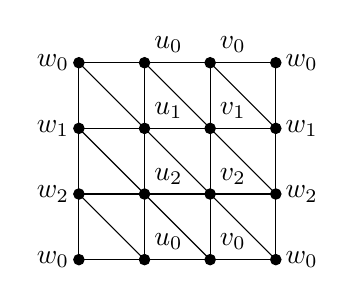
\begin{tikzpicture}[scale=2.5] %Triangulación del Toro
            \coordinate (A) at (0,0);
            \coordinate (B) at (1,0);
            \coordinate (C) at (1,1);
            \coordinate (D) at (0,1);
            
            \coordinate (E) at (1/3,0);
            \coordinate (F) at (2/3,0);
            
            \coordinate (G) at (1,1/3);
            \coordinate (H) at (1,2/3);

            \coordinate (I) at (2/3,1);
            \coordinate (J) at (1/3,1);

            \coordinate (K) at (0,2/3);
            \coordinate (L) at (0,1/3);

            \draw (A) -- (B) -- (C) -- (D) -- cycle;
            
            \draw (E) -- (J);
            \draw (F) -- (I);
            \draw (G) -- (L);
            \draw (H) -- (K);
            
            \draw (E) -- (L);
            \draw (F) -- (K);
            \draw (B) -- (D);
            \draw (H) -- (I);
            \draw (G) -- (J);

            \filldraw (A) circle (0.75pt) node[anchor=east]{$w_{0}$};
            \filldraw (B) circle (0.75pt) node[anchor=west]{$w_{0}$};
            \filldraw (C) circle (0.75pt) node[anchor=west]{$w_{0}$};
            \filldraw (D) circle (0.75pt) node[anchor=east]{$w_{0}$};

            \filldraw (K) circle (0.75pt) node[anchor=east]{$w_{1}$};
            \filldraw (H) circle (0.75pt) node[anchor=west]{$w_{1}$};
            
            \filldraw (L) circle (0.75pt) node[anchor=east]{$w_{2}$};
            \filldraw (G) circle (0.75pt) node[anchor=west]{$w_{2}$};

            \filldraw (E) circle (0.75pt) node[anchor=south west]{$u_{0}$};
            \filldraw (J) circle (0.75pt) node[anchor=south west]{$u_{0}$};
            \filldraw (1/3,2/3) circle (0.75pt) node[anchor=south west]{$u_{1}$};
            \filldraw (1/3,1/3) circle (0.75pt) node[anchor=south west]{$u_{2}$};

            \filldraw (F) circle (0.75pt) node[anchor=south west]{$v_{0}$};
            \filldraw (I) circle (0.75pt) node[anchor=south west]{$v_{0}$};
            \filldraw (2/3,2/3) circle (0.75pt) node[anchor=south west]{$v_{1}$};
            \filldraw (2/3,1/3) circle (0.75pt) node[anchor=south west]{$v_{2}$};
        \end{tikzpicture}
    \end{center}
    es una triangulación.

    \item $\R\mathbb{P}^{2}$ es una superficie triangulable, con
    \begin{center}
        \begin{tikzpicture} %Triangulación del plano proyectivo real
            \filldraw[color=black, fill=white] circle (1.5);

            \coordinate (A) at ({-3*sqrt(3)/4},{3/4});
            \coordinate (B) at ({3*sqrt(3)/4},{3/4});
            \coordinate (C) at (0,-1.5);

            \coordinate (D) at (0,1.5);
            \coordinate (E) at ({-3*sqrt(3)/4},{-3/4});
            \coordinate (F) at ({3*sqrt(3)/4},{-3/4});

            \coordinate (G) at (0,{3/4});
            \coordinate (H) at ({-3*sqrt(3)/8},{-3/8});
            \coordinate (I) at ({3*sqrt(3)/8},{-3/8});

            \draw (A) -- (B) -- (C) -- cycle;
            \draw (G) -- (H) -- (I) -- cycle;
            
            \draw (D) -- (G);
            \draw (E) -- (H);
            \draw (F) -- (I);

            \filldraw (-2,-1.5) node{$N$};

            \filldraw (A) circle (1pt) node[anchor=south east]{$2$};
            \filldraw (B) circle (1pt) node[anchor=south west]{$1$};
            \filldraw (C) circle (1pt) node[anchor=north]{$0$};

            \filldraw (D) circle (1pt) node[anchor=south]{$0$};
            \filldraw (E) circle (1pt) node[anchor=north east]{$1$};
            \filldraw (F) circle (1pt) node[anchor=north west]{$2$};

            \filldraw (G) circle (1pt);
            \filldraw (H) circle (1pt);
            \filldraw (I) circle (1pt);
            
            \filldraw ($(G)-(0,0.1)$) node[anchor=north]{$3$};
            \filldraw ($(H)+(0.1,0)$) node[anchor=south west]{$5$};
            \filldraw ($(I)-(0.1,0)$) node[anchor=south east]{$4$};
        \end{tikzpicture}
    \end{center}
    una triangulación.
\end{itemize}

\noindent A partir de estas superficies podemos construir otras superficies, las sumas conexas. 
Sean $X_{1}$ y $X_{2}$ superficies triangulables. Sean $K_{1},K_{2}$ complejos simpliciales tales
que $\abs{K_{i}}\cong X_{i}$. Consideramos $\varphi_{i}:\Delta^{2}\to \abs{K_{i}}$ encajes 
simpliciales, es decir, $\varphi_{i}$ es un mapeo simplicial tal que $\varphi_{i}(\Delta^{2})$ es 
homeomorfo a un $2-$simplice de $K_{i}$. Consideramos la triangulación de 
$\partial\Delta^{2}\times\Delta^{1}$ como sigue
\begin{center}
    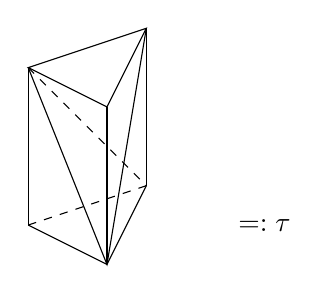
\begin{tikzpicture}%Triangulación del espacio descrito
        \coordinate (A) at (0,0);
        \coordinate (B) at (1,-0.5);
        \coordinate (C) at (1.5,0.5);

        \coordinate (D) at (0,2);
        \coordinate (E) at (1,1.5);
        \coordinate (F) at (1.5,2.5);

        \draw (A) -- (B) -- (C);
        \draw[dashed] (A) -- (C);

        \draw (D) -- (E) -- (F) -- cycle;
        \draw (A) -- (D);
        \draw (B) -- (E);
        \draw (C) -- (F);

        \draw (D) -- (B) -- (F);
        \draw[dashed] (D) -- (C);

        \filldraw (3,0) node{$=:\tau$};
    \end{tikzpicture}
\end{center}
Definimos $X_{1}\#X_{2}$, la suma conexa, como el espacio homeomorfo a $\abs{K_{1}\#K_{2}}$ donde
\begin{equation*}
    K_{1}\#K_{2}:=(K_{1}\setminus\varphi_{1}(\Delta^{2}))\sqcup\tau
    \sqcup(K_{2}\setminus\varphi(\Delta^{2}))/\sim
\end{equation*}
y $\sim$ es tal que $\varphi_{1}(x)\sim(x,0)$ y $\varphi_{2}(x)\sim(x,1)$ para 
$x\in\partial\Delta^{2}$.

\vspace{2mm}
\begin{prop}
    $K_{1}\#K_{2}$ es un complejo simplicial. Mas aún, su realización geométrica, $X_{1}\#X_{2}$
    es una superficie.
\end{prop}

\vspace{2mm}
\begin{dfn}
    Sea $S_{1}:=T^{2}$ y $S_{g}:=S_{g-1}\#T^{2}$ para $g>1$. Del mismo modo, 
    $N_{0}:=\R\mathbb{P}^{2}$ y $N_{g}:=N_{g-1}\#\R\mathbb{P}^{2}$.
\end{dfn}

\noindent Luego, usando Mayer-Vietoris es fácil verificar que
\begin{equation*}
    H_{i}(S_{g})=\begin{cases}
        \Z &\quad\text{si }i=0,2 \\
        \Z^{2g} &\quad\text{si }i=1 \\
        0 &\quad\text{si }i>2
    \end{cases}
    \hspace{2cm}
    H_{i}(S_{g})=\begin{cases}
        \Z &\quad\text{si }i=0 \\
        \Z_{2}\oplus\Z^{g} &\quad\text{si }i=1 \\
        0 &\quad\text{si }i>1
    \end{cases}
\end{equation*}

\begin{teo}[Teorema de Clasificación de Superficies]
    Sean $X,Y$ superficies triangulables compactas. Entonces $X$ es homeomorfa a $Y$ si y solo si
    $H_{i}(X)\cong H_{i}(Y)$ para todo $i$.
\end{teo}

\vspace{2mm}
\begin{dfn}
    Sea $X$ una superficie compacta. Es \textbf{orientable} si $H_{2}(X)\cong\Z$ y es \textbf{no 
    orientable} si $H_{2}(X)\cong0$. El \textbf{género} de una superficie es
    \begin{equation*}
        \begin{cases}
            \frac{rango(H_{1})}{2} &\quad\text{ si es orientable} \\
            rango(H_{2}) &\quad\text{ si no es orientable}
        \end{cases}
    \end{equation*}
\end{dfn}

\vspace{2mm}
\begin{cor}
    Sean $X,Y$ superficies orientables. Entonces $X\cong Y$ si y solo si $\chi(X)=\chi(Y)$.
\end{cor}

\noindent A partir de lo anterior, Poincaré se pregunto si sucedia lo mismo para variedades de
dimensión $3$, en otras palabras $X\cong Y$ si y solo si $H_{i}(X)\cong H_{i}(Y)$ para todo $i$. 
La respuesta es no, el mismo dio un ejemplo. Existe una $3-$variedad $\Sigma$ compacta tal que
$H_{i}(\Sigma)\cong H_{i}(\s^{3})$ que no es homeomorfa a $\s^{3}$.

\vspace{2mm}
\noindent Para distinguir $\Sigma$ de $\s^{3}$ se invento el grupo fundamental.

\newpage
\section{Cohomología}

\subsection{Cohomología Singular}
\begin{dfn}
    Un \textbf{complejo de cocadenas} es una secuencia de grupos de abelianos y homomorfismos
    
    \vspace{2mm}
    \centerline{
        \xymatrix{
            0 \ar[r] & C^{0} \ar[r]^{\partial^{0}} & C^{1} \ar[r]^{\partial^{1}} 
            & C^{2} \ar[r]^{\partial^{2}} & C^{3} \ar[r]^{\partial^{3}} & \cdots
        }
    }

    \vspace{2mm}
    \noindent tales que $\partial^{i+1}\circ\partial^{i}=0$. Se denota por 
    $(C^{\sbullet},\partial^{\sbullet})$.
\end{dfn}

\noindent\textbf{Observación:} Al igual que en complejos de cadenas, los morfismos $\partial^{i}$
se llaman \textbf{diferenciales}, los elementos en $\im{\partial^{i}}$ se dicen 
\textbf{cofronteras} y en $\ker{\partial^{i}}$ se dicen \textbf{cociclos}. Además, es claro que 
$\im{\partial^{i}}\subseteq\kr{\partial^{i+1}}$.

\vspace{2mm}
\begin{dfn}
    El \textbf{$i-$ésimo grupo de cohomología} de $(C^{\sbullet},\partial^{\sbullet})$ se define
    por 
    \begin{equation*}
        H^{i}(C^{\sbullet}):=\frac{\kr{\partial^{i}}}{\im{\partial^{i-1}}}
    \end{equation*}
    Un elemento en $H^{i}(C^{\sbullet})$ se conoce como \textbf{clase de cohomología}.
\end{dfn}

\vspace{2mm}
\noindent\textbf{Ejemplo:} Recordemos el complejo de cadenas

\vspace{2mm}
    \centerline{
        \xymatrix{
            \cdots \ar[r] & 0 \ar[r] & \Z \ar[r]^{\cdot2} & \Z \ar[r]^{\cdot0} & \Z \ar[r] & 0
        }
    }

\vspace{2mm}
\noindent Donde $H_{0}(C_{\sbullet})=\Z$, $H_{1}(C_{\sbullet})=\Z_{2}$ y $H_{k}(C_{\sbullet})=0$. 
Definimos $C^{i}:=Hom(C_{i},\Z)$ y los diferenciales $\partial^{i}(\varphi)
:=\varphi\circ\partial_{i+1}$, notemos que $\partial^{i+1}\circ\partial^{i}(\varphi)
=\varphi\circ\partial_{i+1}\circ\partial_{i+2}=0$. Así, tenemos el complejo de cocadenas

\vspace{2mm}
    \centerline{
        \xymatrix{
            0 \ar[r] & C^{0} \ar[r]^{\cdot0} & C^{1} \ar[r]^{\cdot{2}} & C^{2} \ar[r]^{\cdot0} 
            & 0 \ar[r] & \cdots
        }
    }

\vspace{2mm}
\noindent Como $C^{i}\cong\Z$ para $i=0,1,2$, entonces $H^{0}(C^{\sbullet})=\Z$, 
$H^{1}(C^{\sbullet})=0$ y $H^{2}(C^{\sbullet})=\Z_{2}$.

\vspace{2mm}
\begin{dfn}
    Sean $(C^{\sbullet},\partial^{\sbullet})$ y $(D^{\sbullet},\partial^{\sbullet})$ complejos de
    cocadenas, un \textbf{mapeo de cocadenas}, es una colección $(f^{n})_{n}$ de morfismos
    $f_{n}:C_{n}\to D_{n}$ tales que $\partial^{n}\circ f^{n}=f^{n+1}\circ\partial^{n}$. En otras
    palabras, el diagrama

    \vspace{2mm}
    \centerline{
        \xymatrix{
            C^{n} \ar[r]^{f^{n}} \ar[d]^{\partial^{n}} & D^{n} \ar[d]^{\partial^{n}} \\
            C^{n+1} \ar[r]^{f^{n+1}} & D^{n+1}
        }
    }
    \noindent conmuta.
\end{dfn}

\begin{lema}
    Sea $(f^{n})_{n}$ un mapeo de cocadenas, entonces $f^{*}:H^{n}(C^{\sbullet})\to 
    H^{n}(D^{\sbullet})$ dado por $[x]\to[f^{n}(x)]$ es un morfismo que está bien definido.
\end{lema}

\noindent La demostración de este lema es análoga al caso de complejo de cadenas. Previamente,
definimos el complejo de cadenas singular y los respectivos diferenciales. Usando la idea vista en
el ejemplo vamos a definir la cohomología singular.

\vspace{2mm}
\begin{dfn}
    Sea $X$ un espacio topológico. Definimos los grupos $C^{i}(X):=Hom(C_{i}(X),\Z)$ y los 
    diferenciales $\partial^{i}:C^{i}(X)\to C^{i+1}(X)$ dados por $\partial^{i}(\varphi)
    :=\varphi\circ\partial_{i+1}$. El \textbf{complejo de cocadenas singular} es
    
    \vspace{2mm}
    \centerline{
        \xymatrix{
            0 \ar[r] & C^{0}(X) \ar[r]^{\partial^{0}} & C^{1}(X) \ar[r]^{\partial^{1}} 
            & C^{2}(X) \ar[r]^{\partial^{2}} & C^{3}(X) \ar[r]^{\partial^{3}} & \cdots
        }
    }

    \vspace{2mm}
    \noindent El \textbf{$i-$ésimo grupo de cohomología} esta dado por
    \begin{equation*}
        H^{i}(X):=H^{i}(C^{\sbullet}(X))
    \end{equation*}
\end{dfn}

\noindent\textbf{Observación:} No es cierto en general que $H^{i}(X)=Hom(H_{i}(X),\Z)$, basta 
regresar al ejemplo y notar que $H_{1}(C_{\sbullet})=\Z_{2}\neq0=H^{1}(C^{\sbullet})$.

\newpage
\subsection{Producto Cup}

\newpage
\subsection{Anillo de Cohomología}

\newpage
\subsection{Dualidad de Poincaré y Fórmula de Künneth}

\newpage
\section{Grupo Fundamental}

\subsection{Primer Grupo Fundamental}
\noindent Sea $I=[0,1]$ y $X$ un espacio topológico.

\vspace{2mm}
\begin{dfn}
    Un \textbf{camino} entre $x_{0}$ y $x_{1}$ en $X$ es una función continua $\alpha:I\to X$ tal 
    que $\alpha(0)=x_{0}$ y $\alpha(1)=x_{1}$. Si $\alpha(0)=\alpha(1)=x_{0}$ se dice 
    \textbf{lazo basado} en $x_{0}$.
\end{dfn}

\vspace{2mm}
\noindent Denotamos por $ctx_{0}$ al lazo constante basado en $x_{0}$. Los caminos se pueden 
\textbf{concatenar}, si $\alpha$ y $\beta$ son caminos, entonces
\begin{equation*}
    (\alpha*\beta)(t):=\begin{cases}
        \alpha(2t) &\quad\text{ si}\hspace{2mm}0\leq t\leq\frac{1}{2} \\
        \beta(2t-1) &\quad\text{ si}\hspace{2mm}\frac{1}{2}\leq t\leq1
    \end{cases}
\end{equation*}
es un camino entre $\alpha(0)$ y $\beta(1)$.

\vspace{2mm}
\begin{dfn}
    Una \textbf{homotopía relativa} a $\{0,1\}$ entre caminos $\alpha,\beta:I\to X$ de $x_{0}$ a 
    $x_{1}$ es una homotopía $H:I\times[0,1]\to X$ entre $\alpha$ y $\beta$ tal que $H(0,t)=x_{0}$ 
    y $H(1,t)=x_{1}$ para todo $t\in[0,1]$.
\end{dfn}

\vspace{2mm}
\begin{dfn}
    Sea $X$ un espacio topológico y $x_{0}\in X$. Sea $\pi_{1}(X,x_{0})$ el conjunto de clases de 
    homotopía relativa a $\{0,1\}$ de lazos en $X$ basados en $x_{0}$.
\end{dfn}

\begin{teo}
    Sea $X$ un espacio topológico y $x_{0}\in X$. La operación
    \begin{align*}
        *:\pi_{1}(X,x_{0})\times\pi_{1}(X,x_{0}) &\to \pi_{1}(X,x_{0}) \\
        [\alpha]*[\beta] &\to [\alpha*\beta]
    \end{align*}
    está bien definida y junto con el elemento $e:=[ctx_{0}]$ dan estructura de grupo a 
    $\pi_{1}(X,x_{0})$.
\end{teo}

\begin{proof}
    Debemos probar cuatro puntos
    \begin{itemize}
        \item La operación esta bien definida. Sean $\alpha\sim\alpha'$ y $\beta\sim\beta'$ lazos
        basados en $x_{0}$, entonces $\alpha*\beta\sim\alpha'*\beta'$. Definimos 
        $F:I\times[0,1]\to X$
        \begin{equation*}
            F(s,t):=\begin{cases}
                H(2s,t) &\quad\text{ si}\hspace{4mm}0\leq s\leq\frac{1}{2} \\
                G(2s-1,t) &\quad\text{ si}\hspace{4mm}\frac{1}{2}\leq s\leq1
            \end{cases}
        \end{equation*}
        donde $H$ y $G$ son homotopías relativas entre $\alpha, \alpha'$ y $\beta,\beta'$ 
        respectivamente. Luego, $F(s,0)=(\alpha*\beta)(s)$ y $F(s,1)=(\alpha'*\beta')(s)$, es 
        decir, $F$ es una homología relativa entre $\alpha*\beta$ y $\alpha'*\beta'$.

        \item El elemento $e$ es neutro. Sea $\alpha$ un lazo basado en $x_{0}$. Definimos
        \begin{equation*}
            H(s,t):=\begin{cases}
                \alpha\left(\frac{2s}{t+1}\right) 
                &\quad\text{ si}\hspace{2mm}0\leq s\leq\frac{1}{2} \\
                x_{0} &\quad\text{ si}\hspace{2mm}\frac{1}{2}\leq s\leq1
            \end{cases}
        \end{equation*}
        Es directo que $H$ es una homotopía relativa entre $\alpha*ctx_{0}$ y $\alpha$.

        \item Existencia de inverso. Definimos $\alpha^{-1}(s)=\alpha(1-s)$, por demostrar que
        $[\alpha]*[\alpha^{-1}]=e$, esto es, $\alpha*\alpha^{-1}\sim ctx_{0}$. Definimos
        \begin{equation*}
            H(s,t):=\begin{cases}
                \alpha(2s) &\quad\text{si}\hspace{2mm}0\leq s\leq\frac{1-t}{2} \\
                \alpha(1-t) &\quad\text{si}\hspace{2mm}\frac{1-t}{2} \leq s\leq\frac{1+t}{2} \\
                \alpha^{-1}(2s-1) &\quad\text{si}\hspace{2mm}\frac{1+t}{2}\leq s\leq1
            \end{cases}
        \end{equation*}
        Se verifica que $H$ es una homotopía relativa entre ambos lazos.

        \item Sean $\alpha,\beta,\gamma$ lazos basos en $x_{0}$, entonces la función
        \begin{equation*}
            H(s,t):=\begin{cases}
                \alpha\left(\frac{4s}{1+t}\right) 
                &\quad\text{si}\hspace{2mm}0\leq s\leq\frac{1+t}{4} \\
                \beta\left(4s-1-t\right) 
                &\quad\text{si}\hspace{2mm}\frac{1+t}{4}\leq s\leq\frac{2+t}{4} \\
                \gamma\left(1-4\frac{1-s}{2-t}\right) 
                &\quad\text{si}\hspace{2mm}\frac{2+t}{4}\leq s\leq1
            \end{cases}
        \end{equation*}
        es una homotopía relativa entre $(\alpha*\beta)*\gamma$ y $\alpha*(\beta*\gamma)$.
    \end{itemize}
\end{proof}

\begin{dfn}
    El \textbf{grupo fundamental} de $X$ en $x_{0}$ es $\pi_{1}(X,x_{0})$.
\end{dfn}

\vspace{2mm}
\begin{dfn}
    Un \textbf{espacio punteado} es una tupla $(X,x_{0})$ donde $x_{0}\in X$. Un \textbf{morfismo} 
    entre espacios punteados $(X,x_{0})$ y $(Y,y_{0})$ es una función continua
    \begin{equation*}
        f:X\to Y\htext{tal que}f(x_{0})=y_{0}
    \end{equation*}
    Una \textbf{homotopía punteada} es una homotopía $H$ entre $X$ e $Y$ tal que 
    $H(x_{0},t)=y_{0}$ para todo $t\in[0,1]$.
\end{dfn}

\vspace{2mm}
\noindent\textbf{Observación:} Sea $f$ un morfismo, entonces induce un homomorfismo
\begin{align*}
    f_{*}:\pi_{1}(X,x_{0}) &\to \pi_{1}(Y,y_{0}) \\
    [\alpha] &\to [f\circ\alpha]
\end{align*}
Además, $(f\circ g)_{*}=f_{*}\circ g_{*}$ y $id_{*}=id_{\pi_{1}(X,x_{0})}$, entonces $\pi_{1}$ es
invariante topológico.

\begin{teo}[Invarianza Homotópica]
    Sea $f:X\to Y$ equivalencia homotópica, entonces
    \begin{equation*}
        f_{*}:\pi_{1}(X,x_{0})\to\pi_{1}(Y,f(x_{0}))
    \end{equation*}
    es isomorfismo.
\end{teo}

\begin{lema}
    Sea $\gamma:[0,1]\to X$ camino tal que $\gamma(0)=x_{0}$ y $\gamma(1)=x_{1}$. Entonces la 
    función
    \begin{align*}
        \gamma_{\#}:\pi(X,x_{0}) &\to \pi_{1}(X,x_{1}) \\
        [\alpha] &\to [\gamma^{-1}*\alpha*\gamma]
    \end{align*}
    esta bien definida y es isomorifsmo. Es más, si $\gamma\sim\gamma'$ entonces $\gamma_{\#}
    =\gamma'_{\#}$
\end{lema}

\begin{proof}
    
\end{proof}

\begin{proof} (Teorema)
    
\end{proof}

\begin{dfn}
    Un espacio $X$ se dice simplemente conexo, si es arcoconexo y $\pi_{1}(X,x_{0})=0$ para algún 
    $x_{0}\in X$.
\end{dfn}

%\printbibliography % Quitar el comentado si quiero usar bibliografia

\end{document}